\documentclass[11pt]{article}

\usepackage{amsmath}
\usepackage{amsfonts}
\usepackage{amssymb}
\usepackage{amsthm}
\usepackage{graphicx}
\usepackage{subcaption}
\usepackage[colorinlistoftodos]{todonotes}
\usepackage[colorlinks=true, allcolors=blue]{hyperref}
% \usepackage{showlabels}
\usepackage{palatino}
\usepackage{hyphenat}
\usepackage{thm-restate}
\usepackage{natbib}
\usepackage{setspace}
\onehalfspacing
\usepackage{authblk}

% Line numbers and some weirdness
\usepackage{lineno}
\linenumbers
\newcommand*\patchAmsMathEnvironmentForLineno[1]{%
  \expandafter\let\csname old#1\expandafter\endcsname\csname #1\endcsname
  \expandafter\let\csname oldend#1\expandafter\endcsname\csname end#1\endcsname
  \renewenvironment{#1}%
     {\linenomath\csname old#1\endcsname}%
     {\csname oldend#1\endcsname\endlinenomath}}%
\newcommand*\patchBothAmsMathEnvironmentsForLineno[1]{%
  \patchAmsMathEnvironmentForLineno{#1}%
  \patchAmsMathEnvironmentForLineno{#1*}}%
\AtBeginDocument{%
\patchBothAmsMathEnvironmentsForLineno{equation}%
\patchBothAmsMathEnvironmentsForLineno{align}%
\patchBothAmsMathEnvironmentsForLineno{flalign}%
\patchBothAmsMathEnvironmentsForLineno{alignat}%
\patchBothAmsMathEnvironmentsForLineno{gather}%
\patchBothAmsMathEnvironmentsForLineno{multline}%
}

% commented for arXiv submission
%\usepackage{fancyhdr}
% \fancyhead[R]{ submission intended as Article in Discoveries section of \emph{MBE} }


\graphicspath{ {figures/} }

% http://bytesizebio.net/2013/03/11/adding-supplementary-tables-and-figures-in-latex/
\newcommand{\beginsupplement}{%
        \setcounter{table}{0}
        \renewcommand{\thetable}{S\arabic{table}}%
        \setcounter{figure}{0}
        \renewcommand{\thefigure}{S\arabic{figure}}%
     }

% Commands
\newtheorem{theorem}{Theorem}
\newtheorem{lemma}[theorem]{Lemma}
\newtheorem*{definition}{Definition}

\newcommand{\alphabet}{\mathcal{A}}
\newcommand{\fullAlignment}{\mathbf{Y}}
\newcommand{\alignmentColumn}{\mathbf{y}}
\newcommand{\alignmentColumnRV}{Y}
\newcommand{\siteSplit}{\tilde{y}}
\newcommand{\siteSplitSet}{\mathcal{Y}}
\newcommand{\fullAncestralStates}{\mathbf{H}}
\newcommand{\ancestralStateColumn}{\mathbf{h}}
\newcommand{\ancestralStateColumnRV}{H}
\newcommand{\ancestralSplit}{\tilde{h}}
\newcommand{\ancestralSplitSet}{\mathcal{H}}
\newcommand{\ancestralSplitPartition}{\eta}
\newcommand{\fullAncestralSplitPartitions}{\boldsymbol\eta}

\newcommand{\patternToSplit}{\psi}
\newcommand{\ancestralToSplit}{\xi}

\newcommand{\siteSplitRV}{\Psi}
\newcommand{\ancestralSplitRV}{\Xi}

\newcommand{\nCols}{n}
\newcommand{\nSiteRows}{m}
\newcommand{\nAncestralStateRows}{p}
\newcommand{\nSiteSplits}{q}
\newcommand{\nAncestralSplits}{r}

\newcommand{\shannonDivergence}{\ell^M}

\DeclareMathOperator*{\argmax}{argmax}

\allowdisplaybreaks

\title{Joint maximum-likelihood of phylogeny and ancestral states is not consistent}

\author[1]{David A. Shaw}
\author[2]{Vu C. Dinh}
\author[1]{Frederick A. Matsen IV\thanks{Corresponding author. Email: \url{matsen@fredhutch.org}}}
\affil[1]{Computational Biology Program, Fred Hutchinson Cancer Research Center\\ Seattle, WA, USA}
\affil[2]{Department of Mathematical Sciences, University of Delaware\\ Newark, DE, USA}
\date{}

\begin{document}

\renewcommand{\arraystretch}{1.2} % because otherwise exponents get eaten by \hline

\maketitle
% commented for arXiv submission
%\thispagestyle{fancy}

\begin{abstract}
Maximum likelihood estimation in phylogenetics requires a means of handling unknown ancestral states.
Classical maximum likelihood averages over these unknown intermediate states, leading to provably consistent estimation of the topology and continuous model parameters.
Recently, a computationally-efficient approach has been proposed to jointly maximize over these unknown states and phylogenetic parameters.
Although this method of joint maximum likelihood estimation can obtain estimates more quickly, its properties as an estimator are not yet clear.
We show that this method of jointly estimating phylogenetic parameters along with ancestral states is not consistent in general.
We find a sizeable region of parameter space that generates data on a four-taxon tree for which this joint method estimates a multifurcating topology in the limit of infinite-length sequences by estimating one or more branches to be zero length.
More generally, we show that this joint method only estimates branch lengths correctly on a set of measure zero.
We show empirically that branch length estimates are biased even for short branches, with bias of the same order as the branch lengths themselves.
\end{abstract}

\newpage

\section*{Introduction}

Classical maximum likelihood (ML) estimation in phylogenetics operates by integrating out latent ancestral states at the internal nodes of the tree, obtaining an integrated likelihood \citep{Goldman1990-dk}.
In a recent paper, \citet{Sagulenko2018-xl} suggest using an approximation to ML inference in which the likelihood is maximized jointly across model parameters and ancestral sequences on a fixed topology.
This is attractive from a computational perspective: such joint inference can proceed according to an iterative procedure in which ancestral sequences are first estimated and model parameters are optimized conditional on these estimates.
This latter conditional optimization is simpler and more computationally efficient than optimizing the integrated likelihood.
But is it statistically consistent?

An estimator is said to be statistically consistent if it converges to the generating model with probability one in the large-data limit; existing consistency proofs for maximum likelihood phylogenetics \citep{Allman2008-wd,Chai2011-ff,RoyChoudhury2015-ta} apply only to estimating model parameters when the ancestral sequences have been integrated out of the likelihood.
These proofs do not readily extend to include estimating ancestral states.
Moreover, examples of inconsistency arising from problems where the number of parameters increases with the amount of data \citep{Neyman1948-tt} indicate that joint inference of trees and ancestral states may not enjoy good statistical properties.
In this case those additional parameters are the states of ancestral sequences.
%page 2 section 2.1 at the top of the second column first paragraph second sentence
Although \citet{Sagulenko2018-xl} explicitly warn that the approximation is for the case where ``branch lengths are short and only a minority of sites change on a given branch,'' their work motivates understanding the general properties of such joint inference.
In particular, one would like to know when this approximate technique breaks down for both topology and branch length inference, even when sequence data is ``perfect,'' i.e., is generated without sampling error according to the exact model used for inference.

In this paper, we show that jointly inferring trees and ancestral sequences is not consistent in general.
To do so, we use a binary symmetric model with data generated on a four-taxon tree: we compute closed form solutions to the joint objective function and demarcate a sizeable area of branch lengths in which joint inference is guaranteed to give a multifurcating tree in the case of perfect sequence data with an infinite number of sites by estimating one or more branch lengths to be exactly zero.
We show that, when the topology is known and fixed, joint inference for branch length estimation cannot be consistent except on a set of measure zero (i.e.\ a set that occupies zero volume in parameter space).
Empirically, we find areas where joint inference consistently underestimates interior branch lengths, including regions of short branch length where bias is on the same order as the branch length.

\section*{Phylogenetic maximum likelihood}

Assume the binary symmetric model, namely with a character alphabet $\alphabet=\{0,1\}$ and a uniform stationary distribution \citep{Semple2003-em}.
Let $\nSiteRows$ be the number of tips of the tree, and $\nAncestralStateRows = \nSiteRows-2$ be the number of internal nodes.
We observe $\nCols$ independent and identically distributed samples of character data, i.e., an alignment with $\nCols$ columns, $\fullAlignment=[\alignmentColumn_1,\ldots,\alignmentColumn_\nCols]\in\alphabet^{\nSiteRows\times\nCols}$ distributed as the random variable $\alignmentColumnRV$.
The corresponding unobserved ancestral states are $\fullAncestralStates=[\ancestralStateColumn_1,\ldots,\ancestralStateColumn_\nCols]\in\alphabet^{\nAncestralStateRows\times\nCols}$ and distributed as $\ancestralStateColumnRV$ with each $\ancestralStateColumn_i\in\alphabet^\nAncestralStateRows$.

We parameterize branches on the unique unrooted four-tip phylogenetic tree in ways known as the ``inverse Felsenstein (InvFels)'' tree (Figs.~\ref{fig:farris-fels-top}a and~\ref{fig:farris-fels-top}b) and the ``Felsenstein'' tree (Fig.~\ref{fig:farris-fels-top}c).
The ``inverse Felsenstein'' terminology comes from \citet{Swofford2001-hr}, although it is also called the ``Farris'' tree \citep{Siddall1998-hq, Felsenstein2004}.
In the standard configuration of this tree, the interior branch parameters are equal to the bottom two parameters as in Fig.~\ref{fig:farris-fels-top}a.
We use this standard configuration as our data generating process, though we do not constrain our branch parameters to be equal when optimizing our objective function.

\begin{figure}
\centering
\begin{subfigure}{.32\linewidth}
\centering
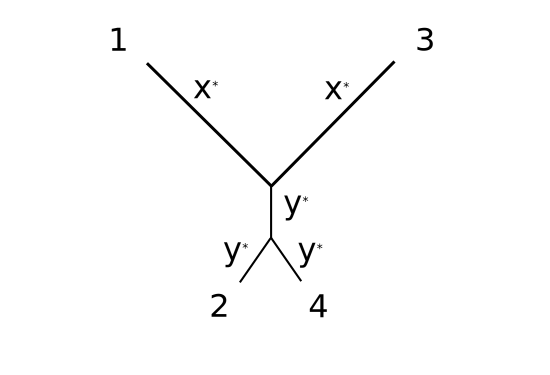
\includegraphics[width=\textwidth]{farris_blank_generating}
\caption[short]{InvFels tree $\tau^*$}
\end{subfigure}
\begin{subfigure}{.32\linewidth}
\centering
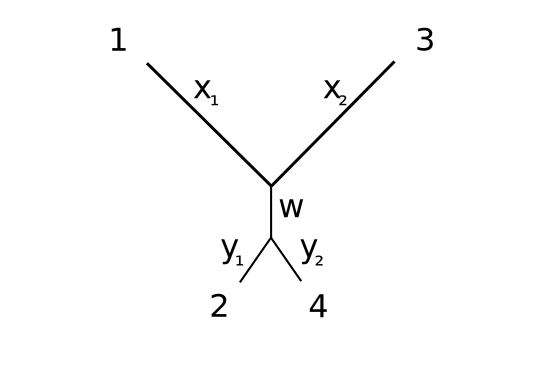
\includegraphics[width=\textwidth]{farris_blank_general}
\caption[short]{InvFels tree $\tau_1$}
\end{subfigure}
\begin{subfigure}{.32\linewidth}
\centering
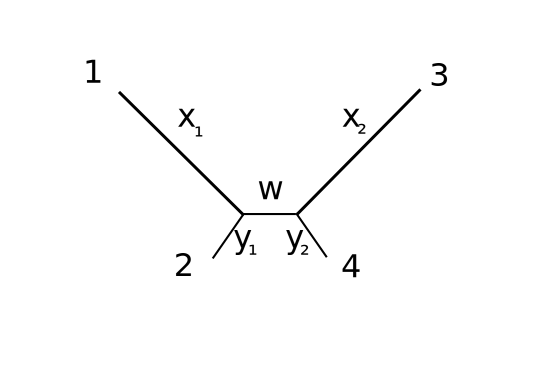
\includegraphics[width=\textwidth]{felsenstein_blank_general}
\caption[short]{Felsenstein tree $\tau_2$}
\end{subfigure}
\caption{Three four-taxon trees with fidelities as labeled.}
\label{fig:farris-fels-top}
\end{figure}

We parameterize the branches of these trees not with the standard notion of branch length in terms of number of substitutions per site, but with an alternate formulation called ``fidelity.''
The probability of a substitution on a branch with fidelity $x$ is $(1-x)/2$, while the probability of no substitution is $(1+x)/2$ where $0 \le x \le 1$.
This parameter quantifies the fidelity of transmission of the ancestral state across an edge \citep{Matsen2007-jq}.

Fidelities have useful algebraic properties.
As data becomes plentiful, we use the Hadamard transform (see \eqref{eq:hadamard_probability} in the Appendix) to compute the exact probabilities that generate each particular configuration of taxa---we call these ``generating probabilities''---and these have an especially simple form.
For a four-taxon tree, define the general branch fidelity parameter $t=\{x_1,y_1,x_2,y_2,w\}$ where fidelities are ordered in the order of the taxa with the internal branch last (Figs.~\ref{fig:farris-fels-top}b and~\ref{fig:farris-fels-top}c).
Although we use fidelities exclusively for our theoretical development, we have made our figures in terms of probabilities of substitution $p_{x} = (1-x)/2$ as they are easier to interpret.

\subsection*{Two paths to maximum likelihood}

The standard phylogenetic likelihood approach on unrooted trees under the usual assumption of independence between sites is as follows.
For a topology $\tau$ and branch fidelities $t$ the likelihood given observed ancestral states $\fullAncestralStates$ is
\begin{equation}
\label{eq:full_likelihood}
L_\nCols(\tau, t; \fullAlignment,\fullAncestralStates) = \prod_{i=1}^{\nCols} \ \Pr(\alignmentColumnRV=\alignmentColumn_i, \ancestralStateColumnRV=\ancestralStateColumn_i \mid \tau, t).
\end{equation}
The probability $\Pr(\alignmentColumnRV=\alignmentColumn_i, \ancestralStateColumnRV=\ancestralStateColumn_i \mid \tau, t)$ is a product of transition probabilities determined by $\fullAlignment$, $\fullAncestralStates$, $\tau$, and $t$ \citep{Felsenstein2004}.

The classical approach is to maximize the likelihood marginalized across ancestral states
\begin{equation}
\label{eq:marginal_likelihood}
\tilde{L}_\nCols(\tau, t; \fullAlignment) = \prod_{i=1}^{\nCols} \ \sum_{\ancestralStateColumn_i\in\alphabet^{\nAncestralStateRows}} \ \Pr(\alignmentColumnRV=\alignmentColumn_i, \ancestralStateColumnRV=\ancestralStateColumn_i \mid \tau, t)
\end{equation}
to estimate the tree $\tau$ and branch fidelities $t$.

The alternative approach \citep{Sagulenko2018-xl} does away with the marginalization and directly estimates the maximum likelihood parameters of the fully-observed likelihood in \eqref{eq:full_likelihood}.
This is known in statistics as a profile likelihood \citep{Murphy2000-ry} or a relative likelihood \citep{Goldman1990-dk}, which exists here because $\alphabet$ is a finite set:
\begin{equation}
\label{eq:profile_likelihood}
L_\nCols'(\tau, t; \fullAlignment) = \prod_{i=1}^{\nCols} \ \max_{\ancestralStateColumn_i\in\alphabet^{\nAncestralStateRows}} \ \Pr(\alignmentColumnRV=\alignmentColumn_i, \ancestralStateColumnRV=\ancestralStateColumn_i \mid \tau, t) = \max_{\fullAncestralStates\in\alphabet^{\nAncestralStateRows\times\nCols}} \ L_\nCols(\tau, t; \fullAlignment, \fullAncestralStates).
\end{equation}
We use $\hat{\fullAncestralStates}_\nCols$ to denote an estimate for $\fullAncestralStates$ obtained by maximizing \eqref{eq:profile_likelihood}, and estimate a topology and branch fidelities using this profile likelihood as
\begin{equation}
\label{eq:profile_likelihood_topology_bl}
(\hat{\tau}_\nCols, \hat{t}_\nCols) = \argmax_{\tau, t} \ L_\nCols'(\tau, t; \fullAlignment).
\end{equation}
In general, the functional form of \eqref{eq:profile_likelihood} is determined by inequalities arising from taking maxima over ancestral states (Table~\ref{tab:farris_likelihoods}) to obtain each conditional likelihood term, these terms depending on the unknown $(\tau, t)$.
For this reason, in practice, the joint inference strategy estimates $\hat{\fullAncestralStates}_\nCols$ for a fixed $(\tau,t)$, then $(\hat{\tau}_\nCols,\hat{t}_\nCols)$ given $\hat{\fullAncestralStates}_\nCols$, maximizing each of these conditional objectives until convergence \citep{Sagulenko2018-xl}.


\section*{Inconsistency of joint inference}

We now state our results on the inconsistency of joint inference.
All proofs are deferred to the Appendix.

Assume $\fullAlignment$ is generated from the InvFels topology $\tau^*$ (Fig.~\ref{fig:farris-fels-top}a) and with true generating branch fidelities $t^*=\{x^*, y^*, x^*, y^*, y^*\}$.
Let $\boldsymbol\xi = [\xi_j]_{j=1}^\nSiteSplits$ be the vector of most likely ancestral state splits---the explicit definition for $\boldsymbol\xi$ is given in the Appendix.
Use $\ell_{\tau^*,t^*}(\tau, t; \boldsymbol\xi)$ to denote the expected per-site log-likelihood, which can be thought of as the infinite-length sequence case because, as shown in the Appendix,
\begin{equation}
\label{eq:exp-log-lik}
\frac{1}{n}\log L_\nCols'(\tau, t; \fullAlignment) \rightarrow \ell_{\tau^*,t^*}(\tau, t; \boldsymbol\xi).
\end{equation}
We give $\ell$ explicitly as \eqref{eq:site_pattern_profile_likelihood_mean} in the Appendix.
For a fixed $\tau$, let $\hat{t}_\nCols$ maximize the left-hand side of \eqref{eq:exp-log-lik} and $\hat{t}$ maximize the right-hand side.
We show in the Appendix that $\hat{t}_\nCols \rightarrow \hat{t}$, allowing us to focus on only the right-hand side above.

%We show that, as $\nCols\rightarrow\infty$, there exist values for $x^*$ and $y^*$ such that the value of the likelihood after maximizing using joint inference is greater for the Felsenstein topology ($\tau_2$) than for the true, generating InvFels topology ($\tau_1$).
%To do so, we construct an upper bound $C_0(x^*, y^*)$ for the likelihood given the InvFels topology as a function of $x^*$ and $y^*$ and, similarly, a lower bound $C_1(x^*, y^*)$ for the likelihood given the Felsenstein topology.
%When $C_0(x^*, y^*) < C_1(x^*, y^*)$, the likelihood in the Felsenstein case is larger than the likelihood in the InvFels case, demonstrating inconsistency (Fig.~\ref{fig:inconsistency-farris}).

\subsection*{Inconsistent branch parameter estimation}
When the topology is known and fixed and we estimate only the branch parameters, we show that for almost all generating parameter values, any branch parameter estimate is consistently biased.
For the branch parameter, we use branch fidelities (discussed earlier) in all statements and proofs, though these trivially extend to branch lengths via transformation.

\begin{restatable}{theorem}{blInconsist}
\label{thm:bl_theorem}
Let $\tau^*=\tau_1$, $t^*=\{x^*, y^*, x^*, y^*, y^*\}$, and $t=\{x_1, y_1, x_2, y_2, w\}$ with $x_1, y_1, x_2, y_2, w > 0$.
For $0 < x^*, y^* < 1$, the solution $\hat{t} := \{\hat{x}_1,\hat{y}_1,\hat{x}_2,\hat{y}_2,\hat{w}\}$ given by
\[
\hat{t} = \arg\max_{t} \ \max_{\boldsymbol\xi} \ \ell_{\tau^*,t^*}(\tau_1, t; \boldsymbol\xi)
\]
has the property that $\hat{t} \neq t^*$ everywhere except a set of measure zero.
\end{restatable}

In words, the joint estimation procedure does not recover the true generating $t^*$ almost everywhere in the space of generating parameters.
The proof can be seen intuitively through the fact that the estimator for a given branch fidelity cannot isolate the individual generating parameter as a linear term since the estimator itself is a combination of nonlinear functions in $(x^*,y^*)$ of generating fidelities.
For example, in estimating $x_1$, $\hat{x}_1$ is a linear combination of $p_{\siteSplit_j}$ values.
For the generating probabilities (top panel of Table~\ref{tab:gen-sitepatprob}), there is no linear combination that results in an isolated $x^*$ term, as all terms are either quadratic, i.e., $(x^*)^2$ or $(x^*)^2(y^*)^2$, or have both $x^*$ and $y^*$, i.e., $x^*(y^*)^2$.
Thus, we cannot obtain a linear combination that in the general case yields $x^*$.
We may have special cases where certain $x^*$ and $y^*$ values yield consistent estimates for $\hat{t}$, but consistency does not hold in general.
We give an example of consistency in a degenerate case in the Appendix following the proof of Theorem~\ref{thm:bl_theorem}.

\subsection*{Convergence to the degenerate topology}
Given data generated on $\tau_1$ there exist true nonzero branch lengths such that the estimator $\hat{t}$ maximizing the right-hand side of \eqref{eq:exp-log-lik} has an internal branch of length zero.
\begin{restatable}{theorem}{topoInconsist}
\label{thm:topo_theorem}
Let $\tau^*=\tau_1$, $t^*=\{x^*, y^*, x^*, y^*, y^*\}$, and $t=\{x_1, y_1, x_2, y_2, w\}$ with $x_1, y_1, x_2, y_2, w > 0$.
There exists an open set of $0 < x^*, y^* < 1$ such that the solution $\hat{t} := \{\hat{x}_1,\hat{y}_1,\hat{x}_2,\hat{y}_2,\hat{w}\}$ given by
\[
\hat{t} = \arg\max_{t} \ \max_{\boldsymbol\xi} \ \ell_{\tau^*,t^*}(\tau_1, t; \boldsymbol\xi)
\]
has the property $\hat{w}\equiv 1$.
\end{restatable}

This result implies an inconsistency because the joint estimate of the interior branch length is zero (i.e., interior branch fidelity is one) in an open set of values for $x^*$ and $y^*$ (Fig.~\ref{fig:bl-general-inconsistency}).
$\hat{w}$ is available in closed form in the entire space of $x^*$ and $y^*$ (table in bottom panel of Fig.~\ref{fig:max-anc-state}).
As we consider different topologies $\tau_1$ and $\tau_2$ for $\hat{t}$, the incorrect topology $\tau_2$ attains a likelihood value at its maximum equal to that of the true topology $\tau_1$ in the limit.
In other words, if $w=1$ the objective functions $\ell_{\tau^*,t^*}(\tau_1, t; \boldsymbol\xi)$ and $\ell_{\tau^*,t^*}(\tau_2, t; \boldsymbol\xi)$ are equivalent.
We elaborate on this point in the Appendix.
The proof is through analytically reducing the general case to 81 separate cases (Table~\ref{tab:likelihoods}) to obtain a closed form maximal value for each.

We provide the following as an intuition for the theoretical development.
For a particular site pattern, to obtain the joint maximum likelihood function we maximize over ancestral states.
For the internal branch---the branch between the two internal nodes---we have a choice of $(1+w)$ or $(1-w)$ in each of our likelihood terms depending on which ancestral state corresponds to the highest conditional log-likelihood.
As $(1+w) > (1-w)$, a maximization procedure tends to prefer the $(1+w)$ term, though this is not guaranteed because the maximum depends on the values of the unknown branch parameters $t$.
Nevertheless, this tendency to include $(1+w)$ terms in the likelihood results in a positive bias of branch fidelities, i.e., estimating branch lengths to be shorter than truth.
This is apparent in the ``long $x^*$, short $y^*$'' scenario as these are the cases in which the most likely ancestral states are the same for each internal node letting $x_1=x_2=x^*$ and $y_1=y_2=y^*$ ($\xi_j=\emptyset$ for all $j$ in Table~\ref{tab:likelihoods}).
If we allow multifurcating trees in our inference, then we can think of this as an instance of converging to the wrong topology, as the true $y^*\neq 1$.

\subsubsection*{Empirical validation}

Direct numerical optimization confirms our theoretically-derived bounds and provides a more detailed picture compared to the analytically\hyp{}derived region (Fig.~\ref{fig:max-anc-state}).
To verify the regions of inconsistency and obtain a clearer picture of the closed form parameter estimates, we plot the optimal $\hat{w}$ via joint estimation (Fig.~\ref{fig:bl-general-inconsistency}).
As before, the region of inconsistency encompasses almost half of the branch fidelity space; given the correct topology, there are many situations where we estimate the interior branch length to be zero.

\begin{figure}
\centering
%file: plotting/_output/invfels/joint_empirical/non-bias/plot.svg
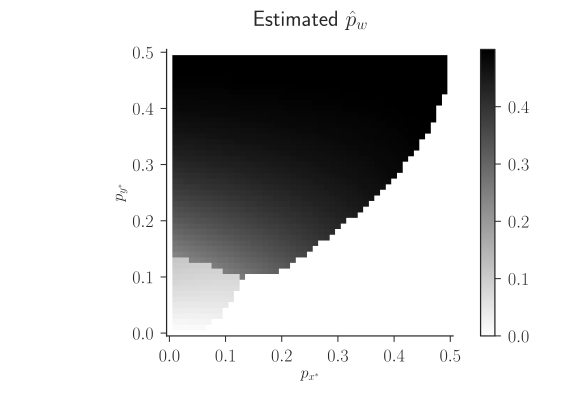
\includegraphics[width=\textwidth]{empirical-estimate}
\caption{
    Estimates for $\hat{p}_w=(1-\hat{w})/2$, the optimal probability of substitution along the inner edge for the profile likelihood \eqref{eq:profile_likelihood}, where the true value for $p_w$ is $p_{y^*}$.
    Regions derived in terms of probabilities of a character change along a branch for ``perfect''data generated on the InvFels topology (Fig.~\ref{fig:farris-fels-top}a).
    The white region in the lower right highlights which values of $x^*$ and $y^*$ result in an interior branch being estimated as length zero, resulting in an inconsistency.
}
\label{fig:bl-general-inconsistency}
\end{figure}

In our optimization procedure, we again consider the 81 separate cases (Table~\ref{tab:likelihoods}) and, for each function, we compute the closed form solution for $\hat{t}$.
We compute these maxima over a lattice in steps of $10^{-2}$ for $x^*,y^*\in(0,1)$.
Our optimization code can be found at \url{https://github.com/matsengrp/joint-inf/}.

In estimating the interior branch length $w$, we find a systematic bias in the joint inference procedure even when the true branches are short (Fig.~\ref{fig:empirical-bias}).
As data are generated with parameters $\{x^*, y^*, x^*, y^*, y^*\}$, the true value for $w$ is $y^*$.
There are discontinuities in the fit (Fig.~\ref{fig:bl-general-inconsistency}) due to the choice of which ancestral state splits are maximal, so we investigate the bias in the region where $p_{x^*}$ and $p_{y^*}$ are both small, i.e., $p_{x^*}, p_{y^*} \le .1$, as these short-branch cases should be the best settings for joint optimization \citep{Sagulenko2018-xl}.
Although the estimates for $\hat{p}_w$ are better than the estimates when $p_{y^*}$ is small and $p_{x^*}$ is large (Fig.~\ref{fig:bl-general-inconsistency}), joint inference still predictably underestimates the interior branch length.
Additionally, the bias estimates $\hat{p}_w-p_{y^*}$ given $p_{x^*}, p_{y^*} \le .1$ are on the same order as the branch lengths (Fig.~\ref{fig:empirical-bias}), showing that even in cases where joint inference is supposed to do well, it still fails to achieve a low error from truth.

In contrast, inference on the integrated likelihood performs as expected, such that $\hat{w}$ is equal to $y^*$ regardless of the value of $x^*$ (Fig.~\ref{fig:bl-general-marginal}).
The errors in this case \eqref{eq:marginal_likelihood} via optimization with L-BFGS-B are lower than machine tolerance.


\begin{figure}
\centering
%file: plotting/_output/invfels/joint_empirical/bias/plot.svg
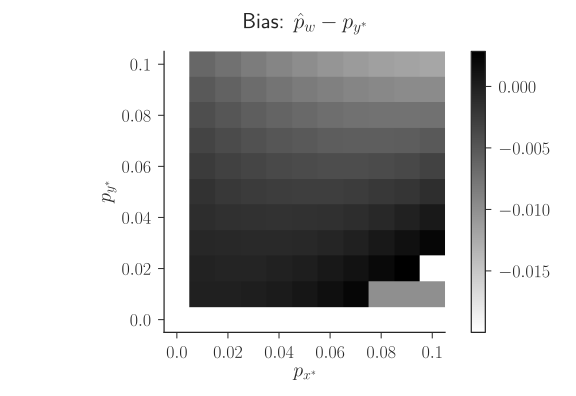
\includegraphics[width=.95\textwidth]{empirical-bias}
\caption{
Bias in branch length estimation.
Even in regions with short branch length ($p_{x^*}, p_{y^*} \le .1$) where joint optimization should perform well, there is systematic bias toward shorter branch lengths.
}
\label{fig:empirical-bias}
\end{figure}

\section*{Discussion}

We have shown that jointly inferring ancestral states and phylogenetic parameters \citep{Sagulenko2018-xl} is not consistent in general.
Specifically, we have shown that the only generating parameters that yield consistent branch length estimates given the correct topology lie in a set of measure zero.
In addition, in the case of four-taxon trees with infinite data, we have obtained nontrivial regions of generating parameters that result in topological ambiguity: the joint inference procedure estimates zero-length branches, which can be considered as a multifurcating topology.
Also, the incorrect topology attains the same likelihood as the topology that generated the data by fixing this branch to have zero length.
Since the parameters with the highest likelihood given the generating topology include a zero-length branch, we cannot exclude the possibility that the incorrect topology with this branch having nonzero length is more likely to be observed, though we have not found regions where this is the case.
The regions of inconsistency we found arise when one set of sister branches of the generating trees are ``long,'' that is, when the top branch fidelities tend to be small, and when the lower branches are ``short,'' i.e., have large fidelities.
We see that this inconsistency occurs even if some branches are short.
This expands on the empirical findings of poor estimation given long branches in \citet{Sagulenko2018-xl} (their Figures~2 and~3).
However, the problems are not just for long branches as \citet{Sagulenko2018-xl} imply: even when all branches are short there is a consistent bias, and the bias is on the same order as the magnitude of the parameters (Fig.~\ref{fig:empirical-bias}).

Joint inference of tree parameters and ancestral sequences is a type of profile likelihood, a well-studied subject in statistics \citep{Murphy2000-ry}.
Many properties regarding the performance of maximum likelihood estimates obtained using this approach are known, and many methods exist to overcome their undesirable properties, e.g., the method of sieves \citep{Geman1982}.
A potential solution in this case using the method of sieves could be to project the column-wise ancestral states into a lower-dimensional space, allowing the degrees of freedom in the ancestral state columns to grow with $\nCols$, albeit more slowly than $O(\nCols)$.
Elsewhere in statistics literature, the failure of maximum likelihood estimates to obtain consistent estimates as the number of parameters goes to infinity have been shown by the Neyman-Scott paradox \citep{Neyman1948-tt}, though parameters tending to infinity is not a necessary condition for inconsistency \citep{LeCam1990}.
Consistency proofs of standard maximum likelihood estimates of phylogeny \eqref{eq:marginal_likelihood} are recent \citep{Allman2008-wd,Chai2011-ff,RoyChoudhury2015-ta}, and no results have been obtained for profile likelihood.
We have furthered progress in understanding the limitations of this joint optimization procedure.

Previous work in phylogenetics has developed consistency counterexamples using similar four-taxon topologies to the one used here \citep{Felsenstein1978-rr}.
In this previous work, when simulating data under the Felsenstein topology $\tau_2$, as the number of observations increases, the InvFels topology $\tau_1$ becomes more likely when performing a particular estimation procedure.
We have shown cases in which, when generating from the InvFels topology, we converge to a multifurcating topology, with one or more branch lengths estimated to be zero.
Moreover, the inconsistency demonstrated by \citet{Felsenstein1978-rr} is attributed to long branch attraction, i.e., the fact that there may be multiple long branches where parallel changes are more likely than a single change along a short branch.
This is not the case here; while analytically the inconsistency occurs on a four-taxon tree when one pair of sister branches are long and the other three are short, we see empirically that this inconsistency is present in roughly half of the entire parameter space, and occurs when the true branches generate data that more likely has no change along the interior branch.
Additionally, we generate data on the InvFels tree $\tau_1$ while \citet{Felsenstein1978-rr} generates data on the Felsenstein tree $\tau_2$.
Difficulties in phylogenetic estimation when generating data on the InvFels tree have been found by \citet{Siddall1998-hq}, though \citet{Swofford2001-hr} show that the difficulties come from insufficient sequence length, which is not the case here.

The case of joint inference of a phylogenetic likelihood is discussed in \citet{Goldman1990-dk}.
There, Goldman provides a worked example in which estimating a topology with fixed branch lengths is equivalent to parsimony and thus not guaranteed to be consistent, though he does not discuss the inconsistency of joint inference in general.
We show cases where the incorrect topology attains an equal likelihood value at the maximum as the correct topology, and, moreover, if we know the correct topology, we show cases where branch lengths are severely biased and cannot be consistent.
Finally, just prior to his conclusion, he discusses when parsimony gives the same answer as maximum likelihood, concluding that the question is ill-posed since parsimony estimates different parameters than maximum likelihood, i.e., it assumes equal branch lengths.
Our question, in contrast, is well-posed: the joint inference procedure outlined here estimates the same parameters as classical maximum likelihood---topology and branch lengths---albeit implicitly estimating ancestral states as well.
We are able to provide much more detail on how large branch lengths must be for general joint inference to fail to be consistent.

%The equal branch length example occurs in Example 2, starting halfway down the second column of page 352 in Goldman (1990) and continuing until the top of the second column on page 354.
%Here he only talks about how parsimony is inconsistent because it may result in equally parsimonious trees (this is the last paragraph of the example section).
%It's not until the bottom of page 356 that he punts the inconsistency to Felsenstein and Hendy/Penny, and the bottom of page 357 where he wonders how small branch lengths have to be for parsimony to be consistent in general.

We have shown an inconsistency when performing joint inference on branch lengths given an InvFels topology and investigated the performance of branch parameter estimation.
There is substantial scope for future work to make these results more precise and more general.
All of these results hold only for a simple binary symmetric model on four-taxon trees, and extensive simulation is necessary to understand how these results extend to more complicated general cases, such as applied examples with larger trees or more realistic mutation models that are of interest to practitioners.
Also, given that many of the bounds presented here are in the form of level sets of multivariate polynomials, a more formal approach using algebraic geometric techniques may reveal more stable or interesting patterns of inconsistency; see \citet{Sturmfels2002} for a thorough treatment of solving systems of polynomial equations.
Finally, all of the material presented here concerns joint estimation under maximum likelihood, and does not pose any problem for other settings, such as joint sampling of trees and ancestral sequences in a Bayesian framework.


\section*{Acknowledgements}
We thank Richard Neher, Vladimir Minin, and Joe Felsenstein for helpful discussions.
Insight from the reviewers and the editors greatly improved this manuscript.

This work was supported by National Institutes of Health grants R01-GM113246, R01-AI120961, U19-AI117891, and U54-GM111274 as well as National Science Foundation grants CISE-1561334 and CISE-1564137.
The research of Frederick Matsen was supported in part by a Faculty Scholar grant from the Howard Hughes Medical Institute and the Simons Foundation.

\bibliographystyle{plainnat}
\bibliography{joint_inf}

\newpage
\beginsupplement

\section*{Appendix}

\subsection*{Site split formulation}
We begin by introducing ``site splits,'' which formalize the notion that a given site pattern is equally probable to its complement under the binary symmetric model.
This is a standard step in the description of the Hadamard transform (Section 8.6 of \citet{Semple2003-em}), although our approach is complicated slightly by the inclusion of ancestral states.

Since we have a finite character alphabet, for a given column $i$ there are a finite number of possible assignments of characters to tips $\alignmentColumn_i$ or internal nodes $\ancestralStateColumn_i$; this results in a simplification of likelihood calculation.
Take the tip labels of $\tau$ to be $\{1,\ldots,\nSiteRows\}$.
For likelihood calculation under the binary symmetric model, we describe a given $\alignmentColumn_i$ as a subset of indices $\siteSplit\subseteq\siteSplitSet:=\{1,\ldots,\nSiteRows-1\}$ with equivalent characters, commonly called a ``site split.''
We define the site split $\siteSplit$ for a $\alignmentColumn_i$ as simply $\alignmentColumn_i$ if the label $\nSiteRows$ is not in $\alignmentColumn_i$, and as its complement otherwise.
Taking such a complement simplifies but does not change the result of likelihood computation because the probability of observing a particular collection of binary characters is equivalent to the probability of its complement under the binary symmetric model.

For topology $\tau$, we define an ordered set of internal node labels $\{1,\ldots,\nAncestralStateRows\}$ for $\ancestralStateColumn_i$ and similarly use a subset of characters $\ancestralSplit\subseteq\ancestralSplitSet:=\{1,\ldots,\nAncestralStateRows\}$ to describe a realization $\ancestralStateColumn_i$.
In this case the entire set of internal nodes must be enumerated: the probability of observing an ancestral state split conditional on a site split is not invariant to taking its complement.

We enumerate the site splits $\siteSplit_j$ of which there are $\nSiteSplits=|\mathcal{P}(\siteSplitSet)|$ in total where $\mathcal{P}$ denotes the power set.
Similarly we enumerate ancestral splits $\ancestralSplit_k$ of which there are $\nAncestralSplits=|\mathcal{P}(\ancestralSplitSet)|$ in total.

We first fix notation.
\begin{definition}
Let the mapping from site patterns to site splits be
$$
\patternToSplit:\alphabet^\nSiteRows\rightarrow\mathcal{P}(\siteSplitSet)
$$
and the mapping from ancestral states and tip states to ancestral state splits be
$$
\ancestralToSplit:\alphabet^\nAncestralStateRows\times\alphabet^\nSiteRows\rightarrow\mathcal{P}(\ancestralSplitSet).
$$
Then, given a site pattern--valued random variable $\alignmentColumnRV$, define the random variable
$$
\siteSplitRV := \patternToSplit(\alignmentColumnRV)
$$
that takes corresponding realizations $\siteSplit_j$ for some $j$, and
$$
\ancestralSplitRV := \ancestralToSplit(\alignmentColumnRV, \ancestralStateColumnRV)
$$
for a tip state--valued random variable $\alignmentColumnRV$ and an ancestral state--valued random variable $\ancestralStateColumnRV$.
\end{definition}
The mapping $\patternToSplit$ takes the complement of site patterns to obtain a site split in $\mathcal{P}(\siteSplitSet)$.
The mapping $\ancestralToSplit$ is defined by whether the tip states have their complements taken or not: if a set of tip labels $\alignmentColumn$ is in $\siteSplitSet$, $\ancestralToSplit(\alignmentColumn, \ancestralStateColumn)$ is $\ancestralStateColumn$; otherwise, if $\alignmentColumn$ is not in $\siteSplitSet$, then the complement of $\alignmentColumn$ necessarily is in $\siteSplitSet$, and $\ancestralToSplit(\alignmentColumn, \ancestralStateColumn)$ is the complement of $\ancestralStateColumn$.

For the $i$th factor of \eqref{eq:full_likelihood},
$$
\Pr(\alignmentColumnRV=\alignmentColumn_i, \ancestralStateColumnRV=\ancestralStateColumn_i \mid \tau, t) = \Pr(\alignmentColumnRV=\alignmentColumn_i \mid \tau, t) \cdot \Pr(\ancestralStateColumnRV=\ancestralStateColumn_i \mid \alignmentColumnRV=\alignmentColumn_i, \tau, t).
$$
As a consequence of assuming a binary symmetric model, taking complements yields
\begin{align*}
    2\cdot \Pr(\alignmentColumnRV=\alignmentColumn_i \mid \tau, t) &= \Pr(\siteSplitRV=\patternToSplit(\alignmentColumn_i) \mid \tau, t) \\
                                                                 &= \Pr(\siteSplitRV=\siteSplit_j \mid \tau, t)
\end{align*}
for some $j$ and
\begin{align*}
    \Pr(\ancestralStateColumnRV=\ancestralStateColumn_i \mid \alignmentColumnRV=\alignmentColumn_i, \tau, t) &= \Pr(\ancestralSplitRV=\ancestralToSplit(\alignmentColumn_i, \ancestralStateColumn_i) \mid \siteSplitRV=\patternToSplit(\alignmentColumn_i), \tau, t).
\end{align*}
Given $(\tau, t)$, there exists an ordered list of sets $\fullAncestralSplitPartitions(\tau, t)=(\ancestralSplitPartition_1(\tau, t),\ldots,\ancestralSplitPartition_\nSiteSplits(\tau, t))$ such that any element $\xi_j$ of the $j$th component $\ancestralSplitPartition_j(\tau, t)$ satisfies
\begin{align*}
\max_{\ancestralSplit_k\in\mathcal{P}(\ancestralSplitSet)} \ \Pr(\ancestralSplitRV=\ancestralSplit_k \mid \siteSplitRV=\siteSplit_j, \tau, t) &= \Pr(\ancestralSplitRV = \xi_j \mid \siteSplitRV=\siteSplit_j, \tau, t).
\end{align*}
In other words, for the $j$th site split, $\ancestralSplitPartition_j(\tau, t)\subset\mathcal{P}(\ancestralSplitSet)$ is the set of most likely ancestral splits for that particular site split, topology and set of branch lengths, and $\xi_j$ is one of possibly many equiprobable ancestral state splits in $\ancestralSplitPartition_j(\tau, t)$.
For each $\alignmentColumn_i$, $\ancestralToSplit(\alignmentColumn_i, \cdot)$ is surjective, and from this we have
\begin{align*}
\max_{\ancestralStateColumn_i} \Pr(\ancestralSplitRV=\ancestralToSplit(\alignmentColumn_i, \ancestralStateColumn_i) \mid \siteSplitRV=\patternToSplit(\alignmentColumn_i), \tau, t) &= \Pr(\ancestralSplitRV = \xi_j \mid \siteSplitRV=\siteSplit_j, \tau, t).
\end{align*}

\subsection*{Site split likelihood}

Let $\xi_j$ be such a choice for each $1 \leq j \leq q$.
Then, the likelihood in \eqref{eq:profile_likelihood} written as a product over site patterns as opposed to sites is
\begin{align}
L_\nCols'(\tau, t; \fullAlignment) &= \max_{\fullAncestralStates} \ L_\nCols(\tau, t; \fullAlignment, \fullAncestralStates) \nonumber \\
                             &= \prod_{i=1}^{\nCols} \ \max_{\ancestralStateColumn_i} \ \Pr(\alignmentColumnRV=\alignmentColumn_i, \ancestralStateColumnRV=\ancestralStateColumn_i \mid \tau, t) \nonumber \\
                             &\propto \prod_{i=1}^{\nCols} \ \max_{\ancestralStateColumn_i} \ \Pr(\siteSplitRV=\patternToSplit(\alignmentColumn_i) \mid \tau, t) \cdot \Pr(\ancestralSplitRV=\ancestralToSplit(\alignmentColumn_i, \ancestralStateColumn_i) \mid \siteSplitRV=\patternToSplit(\alignmentColumn_i), \tau, t) \nonumber \\
                             &= \prod_{i=1}^{\nCols} \ \Pr(\siteSplitRV=\patternToSplit(\alignmentColumn_i) \mid \tau, t) \cdot \max_{\ancestralStateColumn_i} \Pr(\ancestralSplitRV=\ancestralToSplit(\alignmentColumn_i, \ancestralStateColumn_i) \mid \siteSplitRV=\patternToSplit(\alignmentColumn_i), \tau, t) \nonumber \\
                             &= \prod_{j=1}^{\nSiteSplits} \ \left[\Pr(\siteSplitRV=\siteSplit_j \mid \tau, t)\cdot \Pr(\ancestralSplitRV=\xi_j \mid \siteSplitRV=\siteSplit_j, \tau, t)\right] ^{\nCols_j(\fullAlignment)} \label{eq:site_pattern_likelihood}
\end{align}
where $\nCols_j(\fullAlignment)$ is the number of columns in $\fullAlignment$ that project to site split $\siteSplit_j$.

Let
$$
L_\nCols''(\tau, t; \fullAlignment) = \prod_{j=1}^{\nSiteSplits} \ \left[\Pr(\siteSplitRV=\siteSplit_j \mid \tau, t) \cdot \Pr(\ancestralSplitRV=\xi_j \mid \siteSplitRV=\siteSplit_j, \tau, t)\right] ^{\nCols_j(\fullAlignment)}
$$
be the final product in \eqref{eq:site_pattern_likelihood}.
Assume $\nCols$ observations are generated from a model with parameters $(\tau^*, t^*)$.
We have
\begin{equation*}
\begin{split}
&    \frac{1}{\nCols} \log L_\nCols''(\tau, t; \fullAlignment) \\
&\qquad = \sum_{j=1}^\nSiteSplits \frac{\nCols_j(\fullAlignment)}{\nCols}\cdot  \log \Pr(\siteSplitRV=\siteSplit_j, \ancestralSplitRV=\xi_j \mid \tau, t) \\
&\qquad = \sum_{j=1}^\nSiteSplits \frac{\nCols_j(\fullAlignment)}{\nCols}\cdot [\log \Pr(\siteSplitRV=\siteSplit_j \mid \tau, t) +
            \log \Pr(\ancestralSplitRV=\xi_j \mid \siteSplitRV=\siteSplit_j , \tau, t)]
\end{split}
\end{equation*}
so that, in the $\nCols\rightarrow\infty$ limit,
\begin{equation}
\begin{split}
&    \frac{1}{\nCols} \log L_\nCols''(\tau, t; \fullAlignment) \\
&\qquad \rightarrow \sum_{j=1}^\nSiteSplits \Pr(\siteSplitRV=\siteSplit_j \mid \tau^*, t^*) \cdot [\log \Pr(\siteSplitRV=\siteSplit_j \mid \tau, t) + \log \Pr(\ancestralSplitRV=\xi_j \mid \siteSplitRV=\siteSplit_j , \tau, t)]. \label{eq:site_pattern_profile_likelihood_mean}
\end{split}
\end{equation}
Define the divergence quantity
$$
\shannonDivergence_{\tau^*,t^*}(\tau,t) = \sum_{j=1}^\nSiteSplits \Pr(\siteSplitRV=\siteSplit_j \mid \tau^*, t^*)\cdot\log \Pr(\siteSplitRV=\siteSplit_j \mid \tau, t)
$$
and the partial log-likelihood
$$
\tilde{\ell}_{\tau^*,t^*}(\tau, t) = \sum_{j=1}^\nSiteSplits \Pr(\siteSplitRV=\siteSplit_j \mid \tau^*, t^*)\cdot\log \Pr(\ancestralSplitRV=\xi_j \mid \siteSplitRV = \siteSplit_j, \tau, t)
$$
so that \eqref{eq:site_pattern_profile_likelihood_mean} is
\begin{equation}
    \label{eq:log_likelihood_simplified}
    \ell_{\tau^*,t^*}(\tau, t) = \shannonDivergence_{\tau^*,t^*}(\tau,t) + \tilde{\ell}_{\tau^*,t^*}(\tau, t).
\end{equation}

\subsection*{Hadamard representation}

We state the Hadamard representation of site split generating probabilities, following Section 8.6 of \citet{Semple2003-em}.
For each edge $e$ define the edge ``fidelity'' for that edge as
$$
\theta(e) = 1-2p(e).
$$
For an even-sized subset of $Y\subseteq\mathcal{S}$, we define the path set $P(Y)$ as the set of edges in the path connecting both elements of $Y$.
For $n$ taxa, the probability of observing site split $A\in\mathcal{P}(\siteSplitSet)$ is
\begin{equation}
\label{eq:hadamard_probability}
p_A = \frac{1}{2^{n-1}} \ \sum_{Y \subseteq \mathcal{S} : |Y| \equiv 0 (\mathrm{mod} \ 2)} \ \left[(-1)^{|Y \cap A|} \ \prod_{e\in P(Y)} \ \theta(e) \right].
\end{equation}
By convention, we set $P(\emptyset)=\emptyset$ and $\prod_{e\in\emptyset} \ \theta(e) = 1$.
For notational convenience, let
$$
p_{\siteSplit_j} := \Pr(\siteSplitRV=\siteSplit_j \mid \tau_1,t),
$$
for any site split $\siteSplit_j$.
Table~\ref{tab:sitepatprob} contains calculations of site pattern probabilities for our two topologies (Fig.~\ref{fig:farris-fels-top}).

\begin{table}[ht]
\centering
\begin{tabular}{|l|l|l|l|}
    \hline
$\siteSplit_j$  & $p_{\siteSplit_j}$ &$\Pr(\siteSplitRV=\siteSplit_j \mid \tau_1,t)$&$\Pr(\siteSplitRV=\siteSplit_j \mid \tau_2,t)$\\
    \hline
    $\emptyset$ & $p_{\emptyset}$   &$1+x^2+y^2+4xyw+x^2y^2$&$1+2xy+2xyw+x^2w+y^2w+x^2y^2$\\
    $\{1\}$     & $p_{1}$   &$1-x^2+y^2-x^2y^2$&$1-x^2w+y^2w-x^2y^2$\\
    $\{2\}$     & $p_{2}$   &$1+x^2-y^2-x^2y^2$&$1+x^2w-y^2w-x^2y^2$\\
    $\{3\}$     & $p_{3}$   &$1-x^2+y^2-x^2y^2$&$1-x^2w+y^2w-x^2y^2$\\
    $\{1,2\}$   & $p_{12}$   &$1-x^2-y^2+x^2y^2$&$1+2xy-2xyw-x^2w-y^2w+x^2y^2$\\
    $\{1,3\}$   & $p_{13}$   &$1+x^2+y^2-4xyw+x^2y^2$&$1-2xy-2xyw+x^2w+y^2w+x^2y^2$\\
    $\{2,3\}$   & $p_{23}$   &$1-x^2-y^2+x^2y^2$&$1-2xy+2xyw-x^2w-y^2w+x^2y^2$\\
    $\{1,2,3\}$ & $p_{123}$   &$1+x^2-y^2-x^2y^2$&$1+x^2w-y^2w-x^2y^2$\\
    \hline
\end{tabular}
\caption{Site pattern probabilities $p_{\siteSplit_j}$ on the Farris tree $\tau_1$ and the Felsenstein tree $\tau_2$ obtained using the Hadamard transform.
All values multiplied by $1/8$.}
\label{tab:sitepatprob}
\end{table}

\subsection*{Example}
We follow with an expository example computing these probabilities and likelihoods.
Consider the fixed, binary four-taxon tree $\tau_1$ in Fig.~\ref{fig:farris-fels-top}a---this is commonly known as the ``Farris zone'' topology.
The set of all possible character assignments is
\begin{align*}
\mathcal{P}(\{1,2,3,4\}) &= \{\emptyset, \{1,2,3,4\}, \{1\}, \{2,3,4\}, \{2\}, \{1,3,4\}, \{3\}, \{1,2,4\}, \\
                         &\qquad \{1,2\}, \{3,4\}, \{1,3\}, \{2,4\}, \{2,3\}, \{1,4\}, \{1,2,3\}, \{1,4\}\}.
\end{align*}
where each set indicates the tips assigned the character $1$.
For example, $\emptyset$ is the labeling $0000$ and $\{1,3,4\}$ is the labeling $1011$.
Symmetry allows us to group adjacent pairs in $\mathcal{P}(\{1,2,3,4\})$ into equiprobable splits, letting $\siteSplitSet=\{1,2,3\}$.
The unique site splits, collapsing complements, are
\begin{align*}
    \mathcal{P}(\siteSplitSet) &= \{\emptyset, \{1\}, \{2\}, \{3\}, \{1,2\}, \{1,3\}, \{2,3\}, \{1,2,3\}\} \\
& := \{\siteSplit_1, \ldots, \siteSplit_8\}.
\end{align*}
Since we identify character complements, we do not consider the additional splits
\begin{equation*}
\begin{split}
& \mathcal{P}(\{1,2,3,4\}) \setminus \mathcal{P}(\siteSplitSet) = \\
&\qquad \{\{1,2,3,4\}, \{2,3,4\}, \{1,3,4\}, \{1,2,4\}, \{3,4\}, \{2,4\}, \{1,4\}, \{4\}\},
\end{split}
\end{equation*}
the symmetry of the binary character model allowing us to focus only on the elements of $\mathcal{P}(\siteSplitSet)$.
This tree has two internal nodes with $\ancestralSplitSet=\{1,2\}$ and unique ancestral state splits
$$
\mathcal{P}(\ancestralSplitSet) = \{\emptyset, \{1\}, \{2\}, \{1,2\}\}.
$$
Internal node $\{1\}$ is the node connected to leaves $\{1\}$ and $\{3\}$ and internal node $\{2\}$ connected to leaves $\{2\}$ and $\{4\}$.
The mapping from characters to splits in this case will depend on the characters at the tips and the ancestral states.
For example, we take both $\patternToSplit(0000)=\emptyset$ and $\patternToSplit(1111)=\emptyset$.
Similarly, we have $\ancestralToSplit(0000, 00) = \emptyset$ and $\ancestralToSplit(1111, 11)=\emptyset$, needing to take the complement of all the characters present on the tree to identify splits.
We cannot identify complements for ancestral states in the same way as tip states since, for $\siteSplit\in\mathcal{P}(\siteSplitSet)$,
$$
\Pr(\ancestralSplitRV=\emptyset \mid \siteSplitRV=\siteSplit, \tau, t)\neq \Pr(\ancestralSplitRV=\{1,2\} \mid \siteSplitRV=\siteSplit, \tau, t)
$$
in general.

For each site split $\siteSplit\in\mathcal{P}(\siteSplitSet)$, we maximize the likelihood over all $\ancestralSplit\in\mathcal{P}(\ancestralSplitSet)$.
A maximum occurs at one of possibly several ancestral splits in $\mathcal{P}(\ancestralSplitSet)$, defined via $\ancestralSplitPartition_j(\tau, t)$ for the $j$th site split.
As a simple example, say all branch lengths correspond to a probability $p$ ($< 1/2$) of changing character along that branch, with $t=\{p,p,p,p,p\}$.
The probabilities of observing ancestral splits for $\siteSplit_1=\emptyset$ are
$$
\Pr(\ancestralSplitRV=\emptyset \mid \siteSplitRV=\emptyset, \tau, t) =
(1-p)^5,
$$
$$
\Pr(\ancestralSplitRV=\{1\} \mid \siteSplitRV=\emptyset, \tau, t) =
\Pr(\ancestralSplitRV=\{2\} \mid \siteSplitRV=\emptyset, \tau, t) =
p^3(1-p)^2,
$$
$$
\Pr(\ancestralSplitRV=\{1,2\} \mid \siteSplitRV=\emptyset, \tau, t) =
p^4(1-p).
$$
The set of most likely ancestral states contains a single element, here $\ancestralSplitPartition_1(\tau, t)=\{\emptyset\}$.
Then, taking $\xi_1\in\ancestralSplitPartition_1(\tau, t)$ we have
$$
\Pr(\ancestralSplitRV=\xi_1 \mid \siteSplitRV=\emptyset, \tau, t) =
\Pr(\ancestralSplitRV=\emptyset \mid \siteSplitRV=\emptyset, \tau, t) =
(1-p)^5.
$$
For $\siteSplit_5=\{1,2\}$ we have
$$
\Pr(\ancestralSplitRV=\emptyset \mid \siteSplitRV=\{1,2\}, \tau, t) =
\Pr(\ancestralSplitRV=\{1,2\} \mid \siteSplitRV=\{1,2\}, \tau, t) =
p^2(1-p)^3,
$$
$$
\Pr(\ancestralSplitRV=\{1\} \mid \siteSplitRV=\{1,2\}, \tau, t) =
\Pr(\ancestralSplitRV=\{2\} \mid \siteSplitRV=\{1,2\}, \tau, t) =
p^3(1-p)^2.
$$
Here, the set of most likely ancestral states is $\ancestralSplitPartition_5(\tau, t)=\{\emptyset,\{1,2\}\}$, and, for $\xi_5\in\ancestralSplitPartition_5(\tau, t)$,
$$
\Pr(\ancestralSplitRV=\xi_5 \mid \siteSplitRV=\{1,2\}, \tau, t) =
p^2(1-p)^3.
$$

\subsection*{Likelihood computations}

To compute the likelihood of observing a set of data, we need $\Pr(\ancestralStateColumn=\ancestralSplit_k\mid \alignmentColumn=\siteSplit_j,\tau,t)$ for each $\ancestralSplit_k$ and $\siteSplit_j$.
Using branch fidelities, the probability of a character change along a branch with fidelity parameter $\theta$ is $(1-\theta)/2$, while the probability of a character remaining the same is $(1+\theta)/2$.
See Fig.~\ref{fig:example_likelihoods} for the parameters on an example site pattern on the Farris tree.
Likelihood computations for all site patterns and ancestral states are in Tables~\ref{tab:farris_likelihoods} and~\ref{tab:fels_likelihoods}.
Taking maxima row-wise of each table results in Table~\ref{tab:likelihoods}.

\begin{figure}
\centering
\begin{subfigure}{.45\linewidth}
\centering
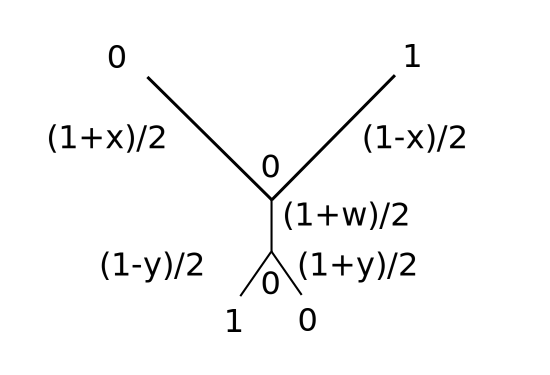
\includegraphics[width=.95\textwidth]{farris_like00}
\caption[short]{}
\end{subfigure}
\begin{subfigure}{.45\linewidth}
\centering
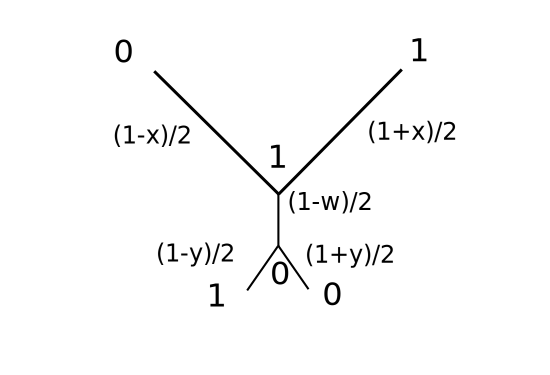
\includegraphics[width=.95\textwidth]{farris_like10}
\caption[short]{}
\end{subfigure}
\caption{
    Example likelihood computations on the Farris tree $\tau_1$ for fidelities $x$, $y$, and $w$.
    Edges labeled by the probability of substitution along that edge.
    In (a), we compute the product to obtain $\Pr(\ancestralStateColumn=\emptyset\mid \alignmentColumn=\{2,3\},\tau_1,t) = (1+x)(1-x)(1+y)(1-y)(1+w)/32$.
    In (b), the same process yields $\Pr(\ancestralStateColumn=\{1\}\mid \alignmentColumn=\{2,3\},\tau_1,t) = (1+x)(1-x)(1+y)(1-y)(1-w)/32$.
}
\label{fig:example_likelihoods}
\end{figure}

\begin{table}
\centering
\begin{tabular}{|l|ll|}
\multicolumn{3}{c}{$\Pr(\ancestralStateColumn=\ancestralSplit_k\mid \alignmentColumn=\siteSplit_j,\tau_1,t)$}\\
\hline
& \multicolumn{2}{|c|}{$\ancestralSplit_k$}\\
    \hline
    $\siteSplit_j$    &$\emptyset$                                &$\{2\}$  \\
    \hline
     $\emptyset$   &$(1+x)^2   (1+w)(1+y)^2$          &$(1+x)^2   (1-w)(1-y)^2$\\
     $\{1\}$       &$(1+x)(1-x)(1+w)(1+y)^2$          &$(1+x)(1-x)(1-w)(1-y)^2$\\
     $\{2\}$       &$(1+x)^2   (1+w)(1+y)(1-y)$       &$(1+x)^2   (1-w)(1+y)(1-y)$\\
     $\{3\}$       &$(1+x)(1-x)(1+w)(1+y)^2$          &$(1+x)(1-x)(1-w)(1-y)^2$\\
     $\{1,2\}$     &$(1+x)(1-x)(1+w)(1+y)(1-y)$       &$(1+x)(1-x)(1-w)(1+y)(1-y)$\\
     $\{1,3\}$     &$(1-x)^2   (1+w)(1+y)^2$          &$(1-x)^2   (1-w)(1-y)^2$\\
     $\{2,3\}$     &$(1+x)(1-x)(1+w)(1+y)(1-y)$       &$(1+x)(1-x)(1-w)(1+y)(1-y)$\\
     $\{1,2,3\}$   &$(1-x)^2   (1+w)(1+y)(1-y)$       &$(1-x)^2   (1-w)(1+y)(1-y)$\\
    \hline
    \hline
    &$\{1\}$                             &$\{1,2\}$  \\
    \hline
     $\emptyset$   &$(1-x)^2   (1-w)(1+y)^2$     &$(1-x)^2   (1+w)(1-y)^2$\\
     $\{1\}$       &$(1+x)(1-x)(1-w)(1+y)^2$     &$(1+x)(1-x)(1+w)(1-y)^2$\\
     $\{2\}$       &$(1-x)^2   (1-w)(1+y)(1-y)$  &$(1-x)^2   (1+w)(1+y)(1-y)$\\
     $\{3\}$       &$(1+x)(1-x)(1-w)(1+y)^2$     &$(1+x)(1-x)(1+w)(1-y)^2$\\
     $\{1,2\}$     &$(1+x)(1-x)(1-w)(1+y)(1-y)$  &$(1+x)(1-x)(1+w)(1+y)(1-y)$\\
     $\{1,3\}$     &$(1+x)^2   (1-w)(1+y)^2$     &$(1+x)^2   (1+w)(1-y)^2$\\
     $\{2,3\}$     &$(1+x)(1-x)(1-w)(1+y)(1-y)$  &$(1+x)(1-x)(1+w)(1+y)(1-y)$\\
     $\{1,2,3\}$   &$(1+x)^2   (1-w)(1+y)(1-y)$  &$(1+x)^2   (1+w)(1+y)(1-y)$\\
    \hline
\end{tabular}
\caption{Likelihood calculations for all site patterns $\siteSplit_j$ and internal states $\ancestralSplit_k$ of the Farris tree $\tau_1$.
All values multiplied by $1/32$.}
\label{tab:farris_likelihoods}
\end{table}

\begin{table}
\centering
\begin{tabular}{|l|ll|}
\multicolumn{3}{c}{$\Pr(\ancestralStateColumn=\ancestralSplit_k\mid \alignmentColumn=\siteSplit_j,\tau_2,t)$}\\
\hline
& \multicolumn{2}{|c|}{$\ancestralSplit_k$}\\
    \hline
    $\siteSplit_j$    &$\emptyset$                                &$\{2\}$  \\
    \hline
     $\emptyset$   &$(1+x)^2   (1+w)(1+y)^2$           &$(1+x)(1-x)(1-w)(1+y)(1-y)$\\
     $\{1\}$       &$(1+x)(1-x)(1+w)(1+y)^2$           &$(1-x)^2   (1-w)(1+y)(1-y)$\\
     $\{2\}$       &$(1+x)^2   (1+w)(1+y)(1-y)$        &$(1+x)(1-x)(1-w)(1-y)^2$\\
     $\{3\}$       &$(1+x)(1-x)(1+w)(1+y)^2$           &$(1+x)^2   (1-w)(1+y)(1-y)$\\
     $\{1,2\}$     &$(1+x)(1-x)(1+w)(1+y)(1-y)$        &$(1-x)^2   (1-w)(1-y)^2$\\
     $\{1,3\}$     &$(1-x)^2   (1+w)(1+y)^2$           &$(1+x)(1-x)(1-w)(1+y)(1-y)$\\
     $\{2,3\}$     &$(1+x)(1-x)(1+w)(1+y)(1-y)$        &$(1+x)^2   (1-w)(1-y)^2$\\
     $\{1,2,3\}$   &$(1-x)^2   (1+w)(1+y)(1-y)$        &$(1+x)(1-x)(1-w)(1-y)^2$\\
    \hline
    \hline
    &$\{1\}$                             &$\{1,2\}$  \\
    \hline
     $\emptyset$   &$(1+x)(1-x)(1-w)(1+y)(1-y)$        &$(1-x)^2   (1+w)(1-y)^2$\\
     $\{1\}$       &$(1+x)^2   (1-w)(1+y)(1-y)$        &$(1+x)(1-x)(1+w)(1-y)^2$\\
     $\{2\}$       &$(1+x)(1-x)(1-w)(1+y)^2$           &$(1-x)^2   (1+w)(1+y)(1-y)$\\
     $\{3\}$       &$(1-x)^2   (1-w)(1+y)(1-y)$        &$(1+x)(1-x)(1+w)(1-y)^2$\\
     $\{1,2\}$     &$(1+x)^2   (1-w)(1+y)^2$           &$(1+x)(1-x)(1+w)(1+y)(1-y)$\\
     $\{1,3\}$     &$(1+x)(1-x)(1-w)(1+y)(1-y)$        &$(1+x)^2   (1+w)(1-y)^2$\\
     $\{2,3\}$     &$(1-x)^2   (1-w)(1+y)^2$           &$(1+x)(1-x)(1+w)(1+y)(1-y)$\\
     $\{1,2,3\}$   &$(1+x)(1-x)(1-w)(1+y)^2$           &$(1+x)^2   (1+w)(1+y)(1-y)$\\
\hline
\end{tabular}
\caption{Likelihood calculations for all site patterns $\siteSplit_j$ and internal states $\ancestralSplit_k$ of the Felsenstein tree $\tau_2$.
All values multiplied by $1/32$.}
\label{tab:fels_likelihoods}
\end{table}

\begin{table}
\centering
\begin{tabular}{|l|ll|}
    \multicolumn{3}{c}{Farris tree ($\tau=\tau_1$)}\\
    \hline
    $\siteSplit_j$    & $\ancestralSplitPartition_j(\tau, t)$ & $\Pr(\ancestralSplitRV=\xi_j \mid \siteSplitRV=\siteSplit_j,\tau,t)$\\
    \hline
    $\emptyset$&
    $\emptyset$&
    $(1+x)^2   (1+w)(1+y)^2$\\
     $\{1\}$    &
    $\emptyset$&
    $(1+x)(1-x)(1+w)(1+y)^2$\\
     $\{2\}$    &
    $\emptyset$&
    $(1+x)^2   (1+w)(1+y)(1-y)$\\
     $\{3\}$    &
    $\emptyset$&
    $(1+x)(1-x)(1+w)(1+y)^2$\\
    $\{1,2\}$  &
    $\{\emptyset,\{1,2\}\}$&
    $(1+x)(1-x)(1+w)(1+y)(1-y)$\\
    $\{1,3\}$  &
    $\left\{\begin{array}{l}
                    \emptyset\\
                    \{1\}\\
                    \{1,2\}
                \end{array}\right.$&
    $\begin{array}{l}
                    (1-x)^2   (1+w)(1+y)^2\\
                    (1+x)^2   (1-w)(1+y)^2\\
                    (1+x)^2   (1+w)(1-y)^2
                \end{array}$\\
    $\{2,3\}$  &
                $\{\emptyset,\{1,2\}\}$&
                $(1+x)(1-x)(1+w)(1+y)(1-y)$\\
    $\{1,2,3\}$&
                $\{1,2\}$&
                $(1+x)^2   (1+w)(1+y)(1-y)$\\
    \hline
    \multicolumn{3}{c}{Felsenstein tree ($\tau=\tau_2$)}\\
    \hline
    $\siteSplit_j$    & $\ancestralSplitPartition_j(\tau, t)$ & $\Pr(\ancestralSplitRV=\xi_j \mid \siteSplitRV=\siteSplit_j,\tau,t)$\\
    \hline
    $\emptyset$       &$\emptyset$&$(1+x)^2   (1+w)(1+y)^2$\\
    $\{1\}$          &
    $\left\{\begin{array}{l}
                    \emptyset\\
                    \{1\}
                \end{array}\right.$&
    $\begin{array}{l}
                        (1+x)(1-x)(1+w)(1+y)^2\\
                        (1+x)^2   (1-w)(1+y)(1-y)
                    \end{array}$\\
      $\{2\}$          &
    $\left\{\begin{array}{l}
                    \emptyset\\
                    \{1\}
                \end{array}\right.$&
    $\begin{array}{l}
                    (1+x)^2   (1+w)(1+y)(1-y)\\
                    (1+x)(1-x)(1-w)(1+y)^2
                    \end{array}$\\
      $\{3\}$          &
    $\left\{\begin{array}{l}
                    \emptyset\\
                    \{2\}
                \end{array}\right.$&
    $\begin{array}{l}
                    (1+x)(1-x)(1+w)(1+y)^2\\
                    (1+x)^2   (1-w)(1+y)(1-y)
                    \end{array}$\\
     $\{1,2\}$         &
    $\left\{\begin{array}{l}
                    \{\emptyset,\{1,2\}\}\\
                    \{1\}
                \end{array}\right.$&
    $\begin{array}{l}
                    (1+x)(1-x)(1+w)(1+y)(1-y)\\
                    (1+x)^2   (1-w)(1+y)^2
                    \end{array}$\\
     $\{1,3\}$         &
    $\left\{\begin{array}{l}
                    \emptyset\\
                    \{\{1\},\{2\}\}\\
                    \{1,2\}
                \end{array}\right.$&
    $\begin{array}{l}
                    (1-x)^2   (1+w)(1+y)^2\\
                    (1+x)(1-x)(1-w)(1+y)(1-y)\\
                    (1+x)^2   (1+w)(1-y)^2
                    \end{array}$\\
      $\{2,3\}$        &
    $\left\{\begin{array}{l}
                    \{\emptyset,\{1,2\}\}\\
                    \{1\}\\
                    \{2\}
                \end{array}\right.$&
    $\begin{array}{l}
                    (1+x)(1-x)(1+w)(1+y)(1-y)\\
                    (1-x)^2   (1-w)(1+y)^2\\
                    (1+x)^2   (1-w)(1-y)^2
                    \end{array}$\\
     $\{1,2,3\}$       &
    $\left\{\begin{array}{l}
                    \{2\} \\
                    \{1,2\}
                \end{array}\right.$&
    $\begin{array}{l}
                    (1+x)(1-x)(1-w)(1+y)^2 \\
                    (1+x)^2   (1+w)(1+y)(1-y)
                    \end{array}$\\
    \hline
\end{tabular}
\caption{Likelihood calculations for all site patterns $\siteSplit_j$ and ancestral state partitions $\ancestralSplitPartition_j$ after maximizing over ancestral states on the Farris tree $\tau_1$ and the Felsenstein tree $\tau_2$.
All values multiplied by $1/32$.
Likelihoods with multiple entries have maxima determined by unknown branch length parameters.
See Tables~\ref{tab:farris_likelihoods} and~\ref{tab:fels_likelihoods} for full calculations.}
\label{tab:likelihoods}
\end{table}

\subsection*{Form of the likelihood}

Consider the Farris tree with arbitrary fidelities, i.e., $\tilde{t}=\{x_1,y_1,x_2,y_2,w\}$.
We now show that, in the case of the Farris tree, exchanging $x_1$ with $x_2$ and $y_1$ with $y_2$ does not change the value of the likelihood, and that constraining both the top two branch parameters to be equal and the bottom two branch parameters to be equal during inference obtains the same maximum likelihood estimate as in the case of arbitrary branch parameters.
Using the Hadamard transform, we calculate the generating probabilities on the Farris tree.
For site split $\emptyset$,
\begin{align*}
    \Pr(\siteSplitRV=\emptyset\mid \tau_1, \tilde{t}) & = \frac{1}{8} (1 + x_1x_2 +  y_1y_2 +  x_1y_1w + x_1y_2w + y_1x_2w + x_2y_2w + x_1y_1x_2y_2) \\
                                              & = \frac{1}{8} (1 + x_1x_2 +  y_1y_2 +  w[x_1y_1 + x_1y_2 + y_1x_2 + x_2y_2] + x_1y_1x_2y_2) \\
                                              & = \frac{1}{8} (1 + x_1x_2 +  y_1y_2 +  w[x_1 + x_2][y_1 + y_2] + x_1y_1x_2y_2).
\end{align*}
and this probability is unchanged when $x_1$ is exchanged with $x_2$ and $y_1$ is exchanged with $y_2$.
All other generating probabilities will differ only in the signs of each term.
For example, for site split $\{1\}$ we have
\begin{align*}
    \Pr(\siteSplitRV=\{1\}\mid \tau_1, \tilde{t}) & = \frac{1}{8} (1 - x_1x_2 +  y_1y_2 +  w[-x_1 + x_2][y_1 + y_2] - x_1y_1x_2y_2)
\end{align*}
and for site split $\{3\}$ we have
\begin{align*}
    \Pr(\siteSplitRV=\{3\}\mid \tau_1, \tilde{t}) & = \frac{1}{8} (1 - x_1x_2 +  y_1y_2 +  w[x_1 - x_2][y_1 + y_2] - x_1y_1x_2y_2)
\end{align*}
meaning if we exchange the values of $x_1$ and $x_2$ then these probabilities swap values.
The corresponding possibilities for the likelihood values are
\begin{align*}
    \Pr(\ancestralSplitRV=\emptyset \mid \siteSplitRV=\{1\}, \tau_1, \tilde{t}) &= \frac{1}{32}(1-x_1)(1+x_2)(1+w)(1+y_1)(1+y_2); \\
    \Pr(\ancestralSplitRV=\{1\} \mid \siteSplitRV=\{1\}, \tau_1, \tilde{t}) &= \frac{1}{32}(1+x_1)(1-x_2)(1-w)(1+y_1)(1+y_2); \\
    \Pr(\ancestralSplitRV=\{2\} \mid \siteSplitRV=\{1\}, \tau_1, \tilde{t}) &= \frac{1}{32}(1-x_1)(1+x_2)(1-w)(1-y_1)(1-y_2); \\
    \Pr(\ancestralSplitRV=\{1,2\} \mid \siteSplitRV=\{1\}, \tau_1, \tilde{t}) &= \frac{1}{32}(1+x_1)(1-x_2)(1+w)(1-y_1)(1-y_2);
\end{align*}
for site split $\{1\}$ and
\begin{align*}
        \Pr(\ancestralSplitRV=\emptyset \mid \siteSplitRV=\{3\}, \tau_1, \tilde{t}) &= \frac{1}{32}(1+x_1)(1-x_2)(1+w)(1+y_1)(1+y_2); \\
    \Pr(\ancestralSplitRV=\{1\} \mid \siteSplitRV=\{3\}, \tau_1, \tilde{t}) &= \frac{1}{32}(1-x_1)(1+x_2)(1-w)(1+y_1)(1+y_2); \\
    \Pr(\ancestralSplitRV=\{2\} \mid \siteSplitRV=\{3\}, \tau_1, \tilde{t}) &= \frac{1}{32}(1+x_1)(1-x_2)(1-w)(1-y_1)(1-y_2); \\
    \Pr(\ancestralSplitRV=\{1,2\} \mid \siteSplitRV=\{3\}, \tau_1, \tilde{t}) &= \frac{1}{32}(1-x_1)(1+x_2)(1+w)(1-y_1)(1-y_2);
\end{align*}
for site split $\{3\}$, which also both swap values when $x_1$ and $x_2$ are exchanged.

The same can be done for the splits $\{2\}$ and $\{1,2,3\}$ by exchanging $y_1$ and $y_2$ as well as $\{1,2\}$ and $\{1,3\}$ by exchanging both $x_1$ with $x_2$ and $y_1$ with $y_2$.
The split $\{1,3\}$ is unchanged by exchanging $x_1$ with $x_2$ and $y_1$ with $y_2$.

Since exchanging $x_1$ and $x_2$ does not change the value of the log-likelihood $\ell_{\tau_1,t^*}(\tau_1, \tilde{t})$, if there is a unique maximum of the log-likelihood we will have $x_1=x_2$ at the maximum.
An analogous statement holds for $y_1$ and $y_2$.
It remains to show that the joint inference procedure maximizing \eqref{eq:profile_likelihood} results in a unique estimate of $t$.
Without loss of generality, we focus on the single parameter $x_1$ and show we obtain a unique maximum when performing joint inference; similar arguments hold for the remaining parameters.
We decompose the likelihood into the entropy and partial likelihood terms as in \eqref{eq:log_likelihood_simplified}.
By Gibbs's inequality, the entropy term $\shannonDivergence_{\tau^*,t^*}(\tau^*,t)$ has a unique maximum over $t$---namely $t^*$.
For the general case of $\tilde{t}=\{x_1, y_2, x_1, y_2, w\}$, we can compute the partial likelihood $\tilde{\ell}_{\tau^*,t^*}(\tau^*, t)$ as in Table~\ref{tab:farris_likelihoods}.
Clearly this partial likelihood will be of the form $g(x_1) = p\log(1+x_1) + (1-p)\log(1-x_1)$ with $0 \le p \le 1$, which, by the second derivative test, is concave for $x_1\in[0,1]$ and thus has a unique maximum.
Since both summands of the likelihood are concave on $x_1\in[0,1]$, the likelihood is as well, and there exists a single $x_1\in[0,1]$ maximizing the likelihood.
Given this and the symmetry of the likelihood, we let $x_1=x_2=x$ and $y_1=y_2=y$.
The Felsenstein tree does not admit this property, but, since we are interested in a lower bound for this tree, we simplify the objective function by constraining $x_1=x_2$ and $y_1=y_2$ similarly.

\subsection*{Theorems and proofs}

\topoInconsist*

\begin{proof}
In general,
$$
\max_{t} \ \ell_{\tau^*,t^*}(\tau, t) \le
    \shannonDivergence_{\tau^*,t^*}(\tau^*,t^*)
    + \tilde{\ell}_{\tau^*,t^*}(\tau, \hat{t})
$$
is an upper bound for the joint maximum of \eqref{eq:log_likelihood_simplified} using Gibbs's inequality
$$
\shannonDivergence_{\tau^*,t^*}(\tau,t) \le \shannonDivergence_{\tau^*,t^*}(\tau^*,t^*)
$$
and
$$
\hat{t} = \argmax_{t} \ \tilde{\ell}_{\tau^*,t^*}(\tau, t).
$$
Similarly,
$$
\max_{t} \ \ell_{\tau^*,t^*}(\tau, t) \ge
    \shannonDivergence_{\tau^*,t^*}(\tau,\hat{t})
    + \tilde{\ell}_{\tau^*,t^*}(\tau, \hat{t})
$$
is a lower bound.

Assume $\tau^*=\tau_1$.
The Farris tree log-likelihood takes one of three values depending on branch lengths, which is due to site split $\{1,3\}$ (see the upper table of Table~\ref{tab:likelihoods}).

We write out the case for the ancestral state split $\{1\}$, and show the other two cases follow a similar argument.
Directly substituting calculations from Table~\ref{tab:sitepatprob} and Table~\ref{tab:likelihoods} where $\tau = \tau_1$ in \eqref{eq:site_pattern_profile_likelihood_mean}, the log-likelihood is, suppressing normalizing constants $-\log 8$ (from the first additive term of \eqref{eq:site_pattern_profile_likelihood_mean}) and $-\log 32$ (from the second),
\begin{align}
    \label{eq:farris_likelihood}
    \ell_{\tau_1,t^*}(\tau_1, t)
    &=        p_{\emptyset}  \cdot\log(1+x^2+y^2+4xyw+x^2y^2) \nonumber \\
    &\qquad + p_{1}          \cdot\log(1-x^2+y^2-x^2y^2) \nonumber \\
    &\qquad + p_{2}          \cdot\log(1+x^2-y^2-x^2y^2) \nonumber \\
    &\qquad + p_{3}          \cdot\log(1-x^2+y^2-x^2y^2) \nonumber \\
    &\qquad + p_{12}         \cdot\log(1-x^2-y^2+x^2y^2) \nonumber \\
    &\qquad + p_{13}         \cdot\log(1+x^2+y^2-4xyw+x^2y^2) \nonumber \\
    &\qquad + p_{23}         \cdot\log(1-x^2-y^2+x^2y^2) \nonumber \\
    &\qquad + p_{123}        \cdot\log(1+x^2-y^2-x^2y^2) \nonumber \\
    &\qquad + p_{\emptyset}  \cdot\log((1+x)^2   (1+w)(1+y)^2) \nonumber \\
    &\qquad + p_{1}          \cdot\log((1+x)(1-x)(1+w)(1+y)^2) \nonumber \\
    &\qquad + p_{2}          \cdot\log((1+x)^2   (1+w)(1+y)(1-y)) \nonumber \\
    &\qquad + p_{3}          \cdot\log((1+x)(1-x)(1+w)(1+y)^2) \nonumber \\
    &\qquad + p_{12}         \cdot\log((1+x)(1-x)(1+w)(1+y)(1-y)) \nonumber \\
    &\qquad + p_{13}         \cdot\log((1+x)^2   (1-w)(1+y)^2) \nonumber \\
    &\qquad + p_{23}         \cdot\log((1+x)(1-x)(1+w)(1+y)(1-y)) \nonumber \\
    &\qquad + p_{123}        \cdot\log((1+x)^2   (1+w)(1+y)(1-y)).
\end{align}
Our plan is to simplify the likelihood to remove log-of-quadratic terms of $x,y,$ and $w$, obtaining a likelihood that has a closed-form maximum in each variable.
To bound the generating probabilities, we use the facts that, for $x,y\in[0,1]$,
\begin{align*}
p_{12} = p_{23} = 1-x^2-y^2+x^2y^2 & = (1+x)(1-x)(1+y)(1-y) \\
p_{1} = p_{3} = 1-x^2+y^2-x^2y^2 & = (1+x)(1-x)(1+y^2) \le (1+x)(1-x)(1+y) \\
p_{2} = p_{123} = 1+x^2-y^2-x^2y^2 & = (1+x^2)(1+y)(1-y) \le (1+x)(1+y)(1-y).
\end{align*}
To bound the remaining $p_{\emptyset}$ and $p_{13}$, we use
\begin{align*}
1+x^2+y^2+x^2y^2 & = (1+x^2)(1+y^2) \le (1+x)(1+y) \\
4xy & = 2x \cdot 2y \le (1+x^2)(1+y^2) \le (1+x)(1+y)
\end{align*}
so that the $p_{\emptyset}$ term is bounded as
\begin{align*}
    p_{\emptyset} & = \log(1+x^2+y^2+4xyw+x^2y^2) \\
                  & \le \log(1+x^2+y^2+4xy+x^2y^2) \\
                  & \le \log(2(1+x)(1+y))
\end{align*}
and $p_{13}$ is bounded as
\begin{align*}
    p_{13} & = \log(1+x^2+y^2-4xyw+x^2y^2) \\
                  & \le \log(1+x^2+y^2+x^2y^2) \\
                  & \le \log((1+x)(1+y)).
\end{align*}
Factoring and making these substitutions (again, under the assumption that the ancestral state split is $\{1\}$) results in
\begin{align*}
&    \ell_{\tau_1,t^*}(\tau_1, t) \\
&\qquad \le      p_{\emptyset}  \cdot\log(2(1+x)(1+y))
+ p_{1}          \cdot\log((1+x)(1-x)(1+y)) \\
    &\qquad\qquad + p_{2}          \cdot\log((1+x)(1+y)(1-y))
+ p_{3}          \cdot\log((1+x)(1-x)(1+y)) \\
    &\qquad\qquad + p_{12}         \cdot\log((1+x)(1-x)(1+y)(1-y))
+ p_{13}         \cdot\log((1+x)(1+y)) \\
    &\qquad\qquad + p_{23}         \cdot\log((1+x)(1-x)(1+y)(1-y))
+ p_{123}        \cdot\log((1+x)(1+y)(1-y)) \\
    &\qquad\qquad + p_{\emptyset}  \cdot\log((1+x)^2   (1+w)(1+y)^2)
+ p_{1}          \cdot\log((1+x)(1-x)(1+w)(1+y)^2) \\
    &\qquad\qquad + p_{2}          \cdot\log((1+x)^2   (1+w)(1+y)(1-y))
+ p_{3}          \cdot\log((1+x)(1-x)(1+w)(1+y)^2) \\
    &\qquad\qquad + p_{12}         \cdot\log((1+x)(1-x)(1+w)(1+y)(1-y))
+ p_{13}         \cdot\log((1+x)^2   (1-w)(1+y)^2) \\
    &\qquad\qquad + p_{23}         \cdot\log((1+x)(1-x)(1+w)(1+y)(1-y))
+ p_{123}        \cdot\log((1+x)^2   (1+w)(1+y)(1-y)) \\
&\qquad =      p_{\emptyset}  \cdot\log(2)
+ \log(1+x)
+ (p_{1}+p_{3}+p_{12}+p_{23})\cdot\log(1-x) \\
&\qquad\qquad + \log(1+y)
+ (p_{2}+p_{12}+p_{23}+p_{123})\cdot\log(1-y) \\
&\qquad\qquad + (2-p_{1}-p_{3}-p_{12}-p_{23})\cdot\log(1+x)
+ (p_{1}+p_{3}+p_{12}+p_{23})\cdot\log(1-x) \\
&\qquad\qquad + (2-p_{2}-p_{12}-p_{23}-p_{123})\cdot\log(1+y)
+ (p_{2}+p_{12}+p_{23}+p_{123})\cdot\log(1-y) \\
&\qquad\qquad + (1-p_{13})\cdot\log(1+w)
+ p_{13}\cdot\log(1-w) \\
&\qquad =      p_{\emptyset}  \cdot\log(2)
+ (3-p_{1}-p_{3}-p_{12}-p_{23})\cdot\log(1+x)
+ 2(p_{1}+p_{3}+p_{12}+p_{23})\cdot\log(1-x) \\
&\qquad\qquad + (3-p_{2}-p_{12}-p_{23}-p_{123})\cdot\log(1+y)
+ 2(p_{2}+p_{12}+p_{23}+p_{123})\cdot\log(1-y) \\
&\qquad\qquad + (1-p_{13})\cdot\log(1+w)
+ p_{13}\cdot\log(1-w).
\end{align*}
To simplify, let
\begin{equation}
    \begin{aligned}
        a_{1} &= 3-p_{1}-p_{3}-p_{12}-p_{23}, \\
        a_{2} &= 2(p_{1}+p_{3}+p_{12}+p_{23}), \\
        a_{3} &= 3-p_{2}-p_{12}-p_{23}-p_{123}, \\
        a_{4} &= 2(p_{2}+p_{12}+p_{23}+p_{123}), \\
    \end{aligned}
    \label{eq:a_const}
\end{equation}
so that
\begin{equation*}
\begin{split}
&    \ell_{\tau_1,t^*}(\tau_1, t) \\
&\qquad \le      p_{\emptyset}  \cdot\log(2)
+ a_{1}\cdot\log(1+x)
+ a_{2}\cdot\log(1-x)
+ a_{3}\cdot\log(1+y) \\
&\qquad\qquad + a_{4}\cdot\log(1-y)
+ (1-p_{13})\cdot\log(1+w)
+ p_{13}\cdot\log(1-w).
\end{split}
\end{equation*}
Maximizing over the unknown terms yields
$$
\hat{x} = \frac{a_{1}-a_{2}}{a_{1}+a_{2}}, \ \hat{y} = \frac{a_{3}-a_{4}}{a_{3}+a_{4}}, \ \hat{w} = 1-2p_{13}.
$$
Trivially $0 \le \hat{w} \le 1$ and $\hat{x}, \hat{y} \le 1$.
We check that $\hat{x}, \hat{y} \ge 0$ to ensure these maxima are valid.
For $\hat{x} \ge 0$ we need $a_1 \ge a_2$; letting
$$
\tilde{p} = p_{1}+p_{3}+p_{12}+p_{23}
$$
we have from \eqref{eq:a_const} that $a_1 \ge a_2$ only if $3 \ge 3\tilde{p}$.
Since $\tilde{p} = 1/8\cdot(4-4(x^*)^2)$, we have $0 \le \tilde{p} \le 1/2$ implying $\hat{x} \ge 0$.
The same approach works for $\hat{y}$.
The upper bound for the likelihood is then maximized at
\begin{align}
\begin{split}
&    \ell_{\tau_1,t^*}(\tau_1, t) \\
&\qquad\le      p_{\emptyset}  \cdot\log(2)
+ a_{1}\cdot\log\frac{2a_{1}}{a_{1}+a_{2}}
+ a_{2}\cdot\log\frac{2a_{2}}{a_{1}+a_{2}}
+ a_{3}\cdot\log\frac{2a_{3}}{a_{3}+a_{4}} \\
&\qquad\qquad + a_{4}\cdot\log\frac{2a_{4}}{a_{3}+a_{4}}
+ (1-p_{13})\cdot\log(2(1-p_{13}))
+ p_{13}\cdot\log(2p_{13}) \\
&\qquad := C^{1}_{\tau_1,\tau_1}(x^*, y^*).
\end{split}
\label{eq:farris-upper-bound}
\end{align}

The other two possible ancestral state splits for the likelihood of the site split $\{1,3\}$ admit similar simplifications.
The upper bound in \eqref{eq:farris-upper-bound} is for the ancestral state split $\{1\}$.
For the ancestral state split $\emptyset$ we see the upper bound will be the same except we lose a $(1+x)^2$ term, gain a $(1-x)^2$ term, lose a $(1-w)$ term, and gain a $(1+w)$ term.
In this case, all terms involving $w$ simplify to $\log(1+w)$, maximized at $\hat{w}=1$.
For the constants above, $a_{1}$ is the multiplier for the $\log(1+x)$ term and $a_{2}$ for the $\log(1-x)$ term meaning that exchanging the above quadratic $x$ terms yields new constants
\begin{equation}
    \begin{aligned}
        a_{1}' &= a_{1}-2p_{13}, \\
        a_{2}' &= a_{2}+2p_{13}, \\
    \end{aligned}
    \label{eq:a_const_prime_x}
\end{equation}
for site split $\emptyset$ and
\begin{equation}
    \begin{aligned}
        a_{3}' &= a_{3}-2p_{13}, \\
        a_{4}' &= a_{4}+2p_{13}, \\
    \end{aligned}
    \label{eq:a_const_prime_y}
\end{equation}
for site split $\{1,2\}$.
To bound the case of $\ancestralSplitPartition_j(\tau_1, t) = \emptyset$,
\begin{align*}
&    \ell_{\tau_1,t^*}(\tau_1, t) \\
&\qquad\le      p_{\emptyset}  \cdot\log(2)
+ a_{1}'\cdot\log\frac{2a_{1}'}{a_{1}'+a_{2}'}
+ a_{2}'\cdot\log\frac{2a_{2}'}{a_{1}'+a_{2}'} \\
&\qquad\qquad + a_{3}\cdot\log\frac{2a_{3}}{a_{3}+a_{4}}
+ a_{4}\cdot\log\frac{2a_{4}}{a_{3}+a_{4}}
+ \log(2) \\
&\qquad := C^{2}_{\tau_1,\tau_1}(x^*, y^*),
\end{align*}
and, for the case of $\ancestralSplitPartition_j(\tau_1, t) = \{1,2\}$,
\begin{align*}
&    \ell_{\tau_1,t^*}(\tau_1, t) \\
&\qquad\le      p_{\emptyset}  \cdot\log(2)
+ a_{1}\cdot\log\frac{2a_{1}}{a_{1}+a_{2}}
+ a_{2}\cdot\log\frac{2a_{2}}{a_{1}+a_{2}} \\
&\qquad\qquad+ a_{3}'\cdot\log\frac{2a_{3}'}{a_{3}'+a_{4}'}
+ a_{4}'\cdot\log\frac{2a_{4}'}{a_{3}'+a_{4}'}
+ \log(2) \\
&\qquad := C^{3}_{\tau_1,\tau_1}(x^*, y^*).
\end{align*}

We now need to check that
$$
\hat{x} = \frac{a_{1}'-a_{2}'}{a_{1}'+a_{2}'}, \ \hat{y} = \frac{a_{3}'-a_{4}'}{a_{3}'+a_{4}'}
$$
are both between zero and one.
Using a similar argument as that where $\ancestralSplitPartition_j(\tau_1, t) = \{1,3\}$, we only need to show $a_1' \ge a_2'$, which is true if $3-2p_{13} \ge 3\tilde{p}+2p_{13}$.
Some rearranging and the fact that $0 \le \tilde{p} \le 1/2$ shows this is equivalent to showing $p_{13} \le 3/8$.
Using Table~\ref{tab:sitepatprob} and $t^*$,
$$
p_{13} = \frac{1}{8}\left(1 + (x^*)^2 + (y^*)^2 - 4x^*(y^*)^2 + (x^*)^2(y^*)^2\right),
$$
meaning we are interested in whether
\begin{equation}
1 + (x^*)^2 + (y^*)^2 - 4x^*(y^*)^2 + (x^*)^2(y^*)^2 \le 3.
\label{eq:generating_ineq}
\end{equation}
We see that
\begin{equation}
1 + (x^*)^2 + (y^*)^2 - 4x^*(y^*)^2 + (x^*)^2(y^*)^2 \le 3 \iff (y^*)^2\left(1 - 4x^* + (x^*)^2\right) \le 2 - (x^*)^2
\label{eq:lenny}
\end{equation}
and that
\begin{align*}
(y^*)^2\left(1 - 4x^* + (x^*)^2\right) &\le (y^*)^2\left(1 - 2x^* + (x^*)^2\right) \\
                                       &=   (y^*)^2\left(1 - x^*\right)^2 \\
                                       &\le        \left(1 - x^*\right)^2 \\
                                       &\le              2 - (x^*)^2,
\end{align*}
with the last inequality holding if $0 \le x^* \le 1$, showing that \eqref{eq:lenny} holds.
Thus, $p_{13} \le 3/8$ and our $\hat{x}$ and $\hat{y}$ are valid.

All bounds are functions only of $x,y$ through the true generating probabilities $x^*, y^*$.
Call the upper bound
$$
C_0(x^*, y^*) := \max\left(C^{1}_{\tau_1,\tau_1}(x^*, y^*), C^{2}_{\tau_1,\tau_1}(x^*, y^*), C^{3}_{\tau_1,\tau_1}(x^*, y^*)\right).
$$

We construct a similar lower bound on the Felsenstein tree partial likelihood.
In the Felsenstein case, there are many more optimal internal states depending on branch lengths than in the Farris case (see the lower table of Table~\ref{tab:likelihoods}).
We first bound the entire likelihood below and then proceed with joint inference.
To obtain a lower bound for the likelihood we replace $1+w$ with $1-w$ in Table~\ref{tab:likelihoods} for $\tau = \tau_2$; in this case, we resolve many of the ambiguous likelihood terms.
For example, for site split $\{1,2\}$, after we replace the $1+w$ term for $\ancestralSplitPartition_j(\tau, t)=\{\emptyset, \{1,2\}\}$ with $1-w$, we have
$$
\max\left((1+x)^2 (1-w)(1+y)^2, (1+x)(1-x)(1-w)(1+y)(1-y)\right)
$$
where since
$$
(1+x)^2 (1-w)(1+y)^2 > (1+x)(1-x)(1-w)(1+y)(1-y),
$$
the maximum for this site split can be bounded below by $(1+x)^2 (1-w)(1+y)^2$.
For the other site splits we consider two cases.
If $(1+x)(1-y) > (1-x)(1+y)$, then
$$
(1+x)^2(1-w)(1+y)(1-y) > (1+x)(1-x)(1-w)(1+y)^2
$$
meaning the cases $\{1\}, \{2\}, \{3\}$ and $\{1,2,3\}$ will have likelihoods bounded below by
$$
(1+x)^2(1-w)(1+y)(1-y).
$$
For the cases $\{1,3\}$ and $\{2,3\}$ and the same condition, we have
$$
(1+x)^2(1-w)(1-y)^2 > (1-x)^2(1-w)(1+y)^2
$$
and
$$
(1+x)^2(1-w)(1-y)^2 > (1+x)(1-x)(1-w)(1+y)(1-y),
$$
yielding lower bounds of
$$
(1+x)^2(1-w)(1-y)^2
$$
in these cases.
The partial likelihood in this case is then bounded below by
\begin{align*}
    \tilde{\ell}_{\tau_1,t^*}(\tau_2, t)
    &\ge      p_{\emptyset}  \cdot\log((1+x)^2   (1-w)(1+y)^2) \\
    &\qquad + p_{1}          \cdot\log((1+x)^2   (1-w)(1+y)(1-y)) \\
    &\qquad + p_{2}          \cdot\log((1+x)^2   (1-w)(1+y)(1-y)) \\
    &\qquad + p_{3}          \cdot\log((1+x)^2   (1-w)(1+y)(1-y)) \\
    &\qquad + p_{12}         \cdot\log((1+x)^2   (1-w)(1+y)^2) \\
    &\qquad + p_{123}        \cdot\log((1+x)^2   (1-w)(1+y)(1-y))\\
    &\qquad + p_{13}         \cdot\log((1+x)^2   (1-w)(1-y)^2) \\
    &\qquad + p_{23}         \cdot\log((1+x)^2   (1-w)(1-y)^2).
\end{align*}
When $(1+x)(1-y) < (1-x)(1+y)$, similar arguments yield the lower bound
\begin{align*}
    \tilde{\ell}_{\tau_1,t^*}(\tau_2, t)
    &\ge      p_{\emptyset}  \cdot\log((1+x)^2    (1-w)(1+y)^2) \\
    &\qquad + p_{1}          \cdot\log((1+x)(1-x)(1-w)(1+y)^2) \\
    &\qquad + p_{2}          \cdot\log((1+x)(1-x)(1-w)(1+y)^2) \\
    &\qquad + p_{3}          \cdot\log((1+x)(1-x)(1-w)(1+y)^2) \\
    %See above.
    &\qquad + p_{12}         \cdot\log((1+x)^2    (1-w)(1+y)^2) \\
    &\qquad + p_{123}        \cdot\log((1+x)(1-x)(1-w)(1+y)^2)\\
    &\qquad + p_{13}         \cdot\log((1-x)^2    (1-w)(1+y)^2) \\
    &\qquad + p_{23}         \cdot\log((1-x)^2    (1-w)(1+y)^2).
\end{align*}
Letting
$$
b = p_{1}+p_{2}+p_{3}+p_{123}
$$
yields
$$
    \tilde{\ell}_{\tau_1,t^*}(\tau_2, t)
    \ge      2\cdot\log(1+x)
    + (2-b)  \cdot\log(1+y)
    + b      \cdot\log(1-y)
    + \log(1-w)
$$
for the first lower bound, and we get the equivalent expression for the second lower bound by exchanging $x$ and $y$.
Maximizing either lower bound over $t$, we obtain
$$
\tilde{\ell}_{\tau_1,t^*}(\tau_2, t)
\ge      2\cdot\log(2)
+ (2-b)  \cdot\log(2-b)
+ b      \cdot\log(b),
$$
i.e., the maximum is achieved at $\{1,1-b,0\}$.
Our lower bound is
$$
C_1(x^*, y^*) := \shannonDivergence_{\tau_1,t^*}(\tau_2,\{1,1-b,0\}) + 2\cdot\log(2) + (2-b)\cdot\log(2-b) + b\cdot\log(b).
$$
See Fig.~\ref{fig:inconsistency-farris} for the values of $0 < x^*, y^* < 1$ where $C_1(x^*, y^*) > C_0(x^*, y^*)$ and joint inference is inconsistent.
\end{proof}

\restrictedBranchInconsist*

\begin{proof}
Recalling Table~\ref{tab:likelihoods} for the Farris tree $\tau = \tau_1$, the likelihood can take one of three forms corresponding to which ancestral state for $\siteSplit_j=\{1,3\}$ maximizes the likelihood over $(x,y,w)$.
If $x=x^*$ and $y=y^*$ are fixed, by collapsing like terms and ignoring terms with only $x^*$ and $y^*$, the log-likelihood in \eqref{eq:farris_likelihood} as a function of $w$ is
\begin{align*}
    \ell_{\tau_1,t^*}(\tau_1, w)
    &\sim     p_{\emptyset}  \cdot\log(1+(x^*)^2+(y^*)^2+4x^*y^*w+(x^*)^2(y^*)^2) \\
    &\qquad + p_{13}         \cdot\log(1+(x^*)^2+(y^*)^2-4x^*y^*w+(x^*)^2(y^*)^2) \\
    &\qquad + (1 - p_{13})\cdot\log(1+w) \\
    &\qquad + p_{13}\cdot\log(1-w)
\end{align*}
where $\sim$ denotes equality up to an additive constant.
Similarly, the other two possibilities for the likelihood both satisfy
\begin{align*}
    \ell_{\tau_1,t^*}(\tau_1, w)
    &\sim     p_{\emptyset}  \cdot\log(1+(x^*)^2+(y^*)^2+4x^*y^*w+(x^*)^2(y^*)^2) \\
    &\qquad + p_{13}         \cdot\log(1+(x^*)^2+(y^*)^2-4x^*y^*w+(x^*)^2(y^*)^2) \\
    &\qquad + \log(1+w).
\end{align*}
Since
$$
\log(1+w) \geq (1 - p_{13})\cdot\log(1+w) + p_{13}\cdot\log(1-w)
$$
with equality only when $w=0$, the second likelihood is the likelihood with the maximum-likelihood ancestral state, and so we only analyze that case.

Now substitute in values for $p_{\emptyset}$ and $p_{13}$ from Table~\ref{tab:sitepatprob}.
Simplifying, the likelihood can be written
$$
\ell(w) = \alpha_1\log(\beta+\gamma w) + \alpha_2\log(\beta-\gamma w) + \log(1+w)
$$
where
$$
\alpha_1 := \alpha_1(x^*, y^*) = \frac{1}{8} \left(1+(x^*)^2+(y^*)^2+4x^*(y^*)^2+(x^*)^2(y^*)^2\right),
$$
$$
\alpha_2 := \alpha_2(x^*, y^*) = \frac{1}{8}\left(1+(x^*)^2+(y^*)^2-4x^*(y^*)^2+(x^*)^2(y^*)^2\right),
$$
$$
\beta := \beta(x^*, y^*) = 1+(x^*)^2+(y^*)^2+(x^*)^2(y^*)^2,
$$
$$
\gamma := \gamma(x^*, y^*) = 4x^*y^*.
$$
Since $x^*$ and $y^*$ fall between zero and one, we make use of the inequalities (excepting the cases of $x^*=y^*=0$ and $x^*=y^*=1$)
$$
\alpha_1 > \alpha_2
$$
and
$$
\beta > \gamma.
$$
% Not sure if I need to show this, but if x and y aren't 1 it's 1+x^2+y^2+x^2y^2 > 4xy => (1+x^2)(1+y^2) > 4xy and 1+x^2 > 2x, 1+y^2 > 2y qed
The derivative of the log-likelihood with respect to $w$ is
$$
\ell'(w) := \frac{d}{dw} \ell(w) = \frac{\alpha_1 \gamma}{\beta+\gamma w} - \frac{\alpha_2 \gamma}{\beta-\gamma w} + \frac{1}{1+w}.
$$
The inequality $\beta > \gamma$ implies that this function stays finite and that, when considering $\ell'(w) \lessgtr 0$, we equivalently consider $f(w) \lessgtr 0$ where $f$ is the quadratic function
\begin{align*}
f(w) &= (w)^2\cdot(-\gamma^2\alpha_1-\gamma^2\alpha_2-\gamma^2) \\
      &\qquad + w\cdot(\gamma\alpha_1\beta-\gamma^2\alpha_1-\gamma\alpha_2\beta-\gamma^2\alpha_2) \\
      &\qquad + (\gamma\alpha_1\beta-\gamma\alpha_2\beta+\beta^2).
\end{align*}
% Note from das: b^2 - 4ac is always \ge 0 by \alpha_1 > \alpha_2, so b^2 - 4ac can only be zero if b is zero and a or c is zero. c is never zero, so this means a must be zero for this to happen, which only occurs if \gamma = 0, i.e., if x or y is zero.
Excepting all the cases where $x^*=0$ or where $y^*=0$, this implies $\ell'$ has two zeros according to the quadratic formula.
Because $\alpha_1 > \alpha_2$ we have $\ell'(0) > 0$, and thus $\ell$ is increasing at $w=0$.
This implies that if the smaller of the zeros of $f(w)$ is greater than one, then $\hat{w} \equiv 1$.
Using the quadratic formula with
$$
a = -\gamma^2 \alpha_1 - \gamma^2 \alpha_2 - \gamma^2,
$$
$$
b = \gamma \alpha_1 \beta - \gamma^2\alpha_1 - \gamma \alpha_2 \beta - \gamma^2 \alpha_2,
$$
$$
c = \gamma \alpha_1 \beta - \gamma \alpha_2 \beta + \beta^2,
$$
the smaller zero is
$$
\hat{w} = \frac{-b - \sqrt{b^2 - 4ac}}{2a},
$$
which is a function of the generating parameters $x^*$ and $y^*$.
We see that $a \le 0$ and, by a small calculation, $2a+b \leq 0$.
With this we have,
$$
\hat{w} \ge 1 \iff
|2a + b| \leq \sqrt{b^2 - 4ac} \iff
%-b - \sqrt{b^2 - 4ac} \le 2a,
%0 \ge -b - 2a \le \sqrt{b^2 - 4ac},
%b^2 + 4ab + 4a^2 \le b^2 - 4ac,
%a^2 + ab + ac \le 0,
a + b + c \ge 0.
$$
Using
$$
\alpha_1 + \alpha_2 = \frac{1}{4}\beta
$$
and
$$
\alpha_1 - \alpha_2 = x^*(y^*)^2,
$$
and simplifying as functions of $\gamma$ and $\beta$ shows that $a + b + c \ge 0$ is equivalent to
\begin{equation}
\label{eq:restricted-bl-result}
%\beta^2-\gamma^2-2\gamma^2\alpha_1-2\gamma^2\alpha_2+2\gamma\alpha_1\beta-2\gamma\alpha_2\beta \ge 0.
-\gamma^2\left(1 + \frac{1}{2}\beta\right) + 2\gamma\beta x^*(y^*)^2 + \beta^2 \ge 0.
\end{equation}
\end{proof}

\generalBranchInconsist*

\begin{proof}
In the general case, $\hat{w}$ is a function of $x^*$, $y^*$, $\hat{x}$, and $\hat{y}$.
From the previous section, $\hat{w}$ is given by the quadratic formula, though now with $\gamma$ and $\beta$ as functions of $\hat{x}$ and $\hat{y}$ instead of $x^*$ and $y^*$.
Assume we know $\hat{x}$ and $\hat{y}$ as functions of $x^*$ and $y^*$ only.
The same derivation as for \eqref{eq:restricted-bl-result} further yields
\begin{equation}
\label{eq:general-bl-result}
-\gamma^2(\hat{x}, \hat{y})\left(1 + \frac{1}{2}\beta\right) + 2\gamma(\hat{x}, \hat{y})\beta(\hat{x}, \hat{y})x^*(y^*)^2 + \beta^2(\hat{x}, \hat{y}) \ge 0
\end{equation}
where, since $\alpha_1$ and $\alpha_2$ are still functions of $x^*$ and $y^*$, $\left(1+1/2\cdot\beta\right)$ and $x^*(y^*)^2$ from \eqref{eq:restricted-bl-result} remain unchanged.
Given the bounds
$$
\gamma_{L} \le \gamma(\hat{x}, \hat{y}) \le \gamma_{U}
$$
and
$$
\beta_{L} \le \beta(\hat{x}, \hat{y}),
$$
if
$$
-\gamma_{U}^2\left(1 + \frac{1}{2}\beta\right) + 2\gamma_{L}\beta_{L}x^*(y^*)^2 + \beta_{L}^2 \ge 0,
$$
then \eqref{eq:general-bl-result} holds, and this is an inequality involving only $x^*$ and $y^*$.
\end{proof}
To get a sense of the region of overestimation, Fig.~\ref{fig:bl-loose-inconsistency} plots an intermediate case.
\subsection*{Empirical validation}

We use basin-hopping \citep{Wales1997} implemented in \texttt{scipy} \citep{Jones2001} to obtain the plots in Figs.~\ref{fig:bl-general-inconsistency}, \ref{fig:bl-general-marginal}, and \ref{fig:bl-general-bias}.
This method randomly perturbs candidate solutions and accepts or rejects them based on the nearby likelihood surface, eventually obtaining an estimate of the ``global'' optimum.
While it is not guaranteed to always obtain a global optimum---or even always converge---its implementation here leads us to believe that we can estimate $\hat{w}$ as well as any optimization method available.

We take various safeguards to ensure convergence and stability of the procedure.
Since this method involves randomness, we take precautions to not evaluate the likelihood near or outside of boundary conditions, i.e., when $x^*$ or $y^*$ are either $0$ or $1$.
As is apparent from Table~\ref{tab:sitepatprob}, if $0 < x^*, y^* < 1$ and we try to evaluate the candidate $\hat{x}=\hat{y}=\hat{w}=1$ we have a likelihood of exactly zero.
Worse still, in Table~\ref{tab:likelihoods} for the Farris tree, in the cases of $\{2\}, \{1,2\}, \{2,3\},$ and $\{1,2,3\}$, any attempt to evaluate $\hat{y}=1$ will similarly yield a zero likelihood.
In these cases of zero likelihood, methods that evaluate many candidate parameter values can fail to converge when near these boundaries.
We sidestep these computational issues by restricting ourselves to the region $x^*,y^*\in [10^{-2},1-10^{-2}]^2$.

We initialize our optimization procedure at the true branch parameters $t^*=\{x^*,y^*,x^*,y^*,y^*\}$.
Because our analysis shows that $\hat{w}$ can be equal to one when $x^*$ and $y^*$ are small, and local optimization may have a hard time obtaining this value if our initial guess is small, we perform two maximizations, one with $w=1$ fixed and one where $w$ is estimated.
We take the value of $\hat{w}$ with the larger objective function as our estimate.

\begin{figure}
\centering
% obtained by running
% python joint_inf_plot.py --empirical --general-branch-lengths --delta .01 --plot-name figures/w-hat-empirical-01-marginal.svg --out-pkl-name figures/w-hat-empirical-01-marginal.pkl --n-jobs 16 --marginal
% or
% python joint_inf_plot.py --empirical --general-branch-lengths --plot-name figures/w-hat-empirical-01-marginal.svg --in-pkl-name figures/w-hat-empirical-01-marginal.pkl
% if fit already
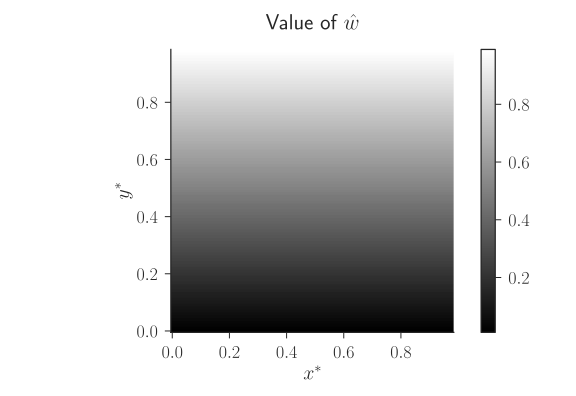
\includegraphics[width=\textwidth]{w-hat-empirical-01-marginal}
\caption{
    Estimates for $\hat{w}$ when computing $(\hat{x}, \hat{y}, \hat{w})$ using basin-hopping \citep{Wales1997} optimizing the classical marginal likelihood \eqref{eq:marginal_likelihood} (rather than a joint optimization procedure).
}
\label{fig:bl-general-marginal}
\end{figure}

\begin{figure}
\centering
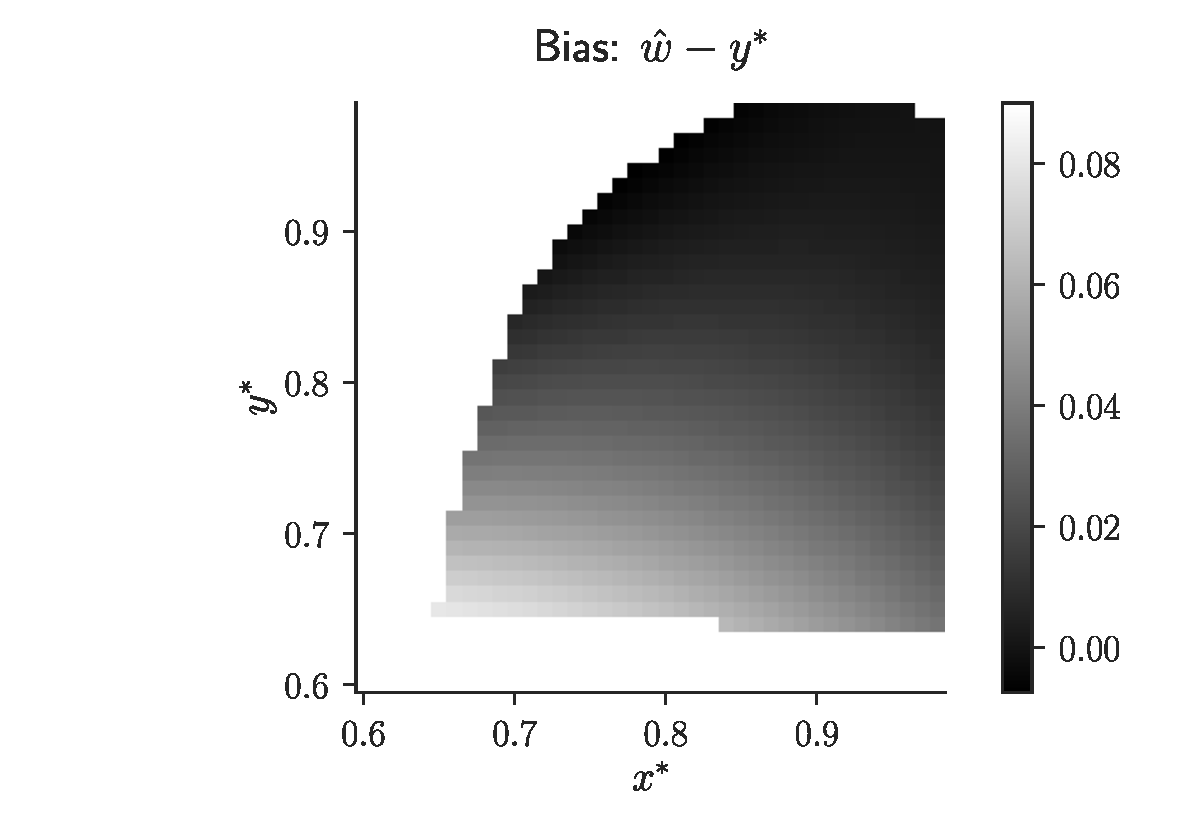
\includegraphics[width=\textwidth]{w-hat-empirical-01-bias}
\caption{
    Estimates for $\hat{w}-y^*$ when computing $(\hat{x}, \hat{y}, \hat{w})$ using basin-hopping \citep{Wales1997} optimizing \eqref{eq:profile_likelihood}.
    Plot focuses on $0.6 < x^*, y^* < 1$ where $\hat{w}$ is estimated to be a value different from 1.
    We do not compute the bias for the white region where $\hat{w}=1$ to preserve a useful scale for the rest of the plot.
}
\label{fig:bl-general-bias}
\end{figure}



\end{document}
